%-----------------------------------------------------------------------------%
\chapter{\babLima}
\label{bab:5}
%-----------------------------------------------------------------------------%
% This chapter explains and analyzes the results of the testing done according to the application infrastructure, test scenarios, and evaluation metrics that have been defined.
This chapter discusses the test results and analysis. The discussion includes reliability analysis and performance analysis.

% It seems that the MCS with MCI approach has better performance, which is especially shown during low traffic conditions during the 10 requests / second experiment, where the MCS with MCI approach had no server failures which subsequently causes it to be restarted, while the Istio / ASM have restarted multiple times during the test done in the smallest requests per second variable.


%-----------------------------------------------------------------------------%
\section{Reliability}
\label{sec:analisis}
To evaluate the reliability of geo-distributed clusters, we tested the single-cluster variation as well for comparison. In addition, analyzing the single-cluster results also helps us understand the behavior of each geo-distributed cluster method, mainly its recovery and failover mechanism.

After configuring and testing each scenario, the results can be seen in \autoref{tab:reliability-single-cluster-results} and \autoref{tab:reliability-multi-cluster-results} for single cluster and multi-cluster test results, respectively. The main result that determines reliability is the success ratio for each method.

\begin{table}[h]
\centering
\caption{Single Cluster Reliability Test Results}

\begin{tabular}{|c|c|c|c|}
\hline

\textbf{Method} & \textbf{Location} & \textbf{RPS} & \textbf{Success Ratio} \\ \hline
%  &  &  & \textbf{Min} & \textbf{Mean} & \textbf{Max} &  \\ \hline
%  & & 10 & 2.771 & 3.72 & 6.867 & 100.00\% \\ \cline{3-7}
%  & southeast-asia & 50 & 2.71 & 3.761 & 18.27 & 100.00\% \\ \cline{3-7}
% MCS with & & 100 & 2.546 & 3.851 & 20.348 & 100.00\% \\ \cline{2-7}
% MCI & & 10 & 3.571 & 4.879 & 10.445 & 100.00\% \\ \cline{3-7}
%  & australia & 50 & 3.33 & 4.55 & 14.095 & 100.00\% \\ \cline{3-7}
%  & & 100 & 3.29 & 4.623 & 17.547 & 100.00\% \\ \hline
%  & & 10 & 1.745 & 3.709 & 52.527 & 62.67\% \\ \cline{3-7}
%  & southeast-asia & 50 & 1.512 & 3.232 & 35.926 & 71.87\% \\ \cline{3-7}
% Istio / & & 100 & 1.426 & 2.912 & 44.033 & 71.93\% \\ \cline{2-7}
% ASM & & 10 & 1.783 & 32.38 & 127.82 & 33.33\% \\ \cline{3-7}
%  & australia & 50 & 1.696 & 10.959 & 114.222 & 34.67\% \\ \cline{3-7}
%  & & 100 & 1.453 & 7.383 & 289.035 & 30.07\% \\ \hline

 & & 10 & 100.00\% \\ \cline{3-4}
 & southeast-asia & 50 & 100.00\% \\ \cline{3-4}
MCS with & & 100 & 100.00\% \\ \cline{2-4}
MCI & & 10 & 100.00\% \\ \cline{3-4}
 & australia & 50 & 100.00\% \\ \cline{3-4}
 & & 100 & 100.00\% \\ \hline
 & & 10 & 62.67\% \\ \cline{3-4}
 & southeast-asia & 50 & 71.87\% \\ \cline{3-4}
Istio / & & 100 & 71.93\% \\ \cline{2-4}
ASM & & 10 & 33.33\% \\ \cline{3-4}
 & australia & 50 & 34.67\% \\ \cline{3-4}
 & & 100 & 30.07\% \\ \hline

\end{tabular}
\label{tab:reliability-single-cluster-results}
\end{table}

From the single cluster test results, it can be seen that MCS with MCI performs better than Istio / ASM as it is able to handle up to 100 requests per second. This can be explained by the added complexity that Istio brings inside of a Kubernetes architecture, mainly having to inject the Envoy sidecar in each pod. This results in more resources and time required, especially in the case of server recovery during high traffic. In addition, the error response set, as seen in \autoref{pic:error-code-0}, confirms this, as all of the errors have a response code of 0, which means that the requests weren't sent at all, as the server was busy restarting. Server restarts are an expected behavior, as it happens when a server is overloaded, as indicated by an error response code, and are necessary to return a server to a healthy state. Furthermore, the internal state of the pod can be seen in \autoref{pic:readiness-probe-fail}, where a readiness probe, which is done to check if a pod is healthy, failed as it has not recovered. This results in the connection refused error received by the client.

\begin{figure}
	\centering
	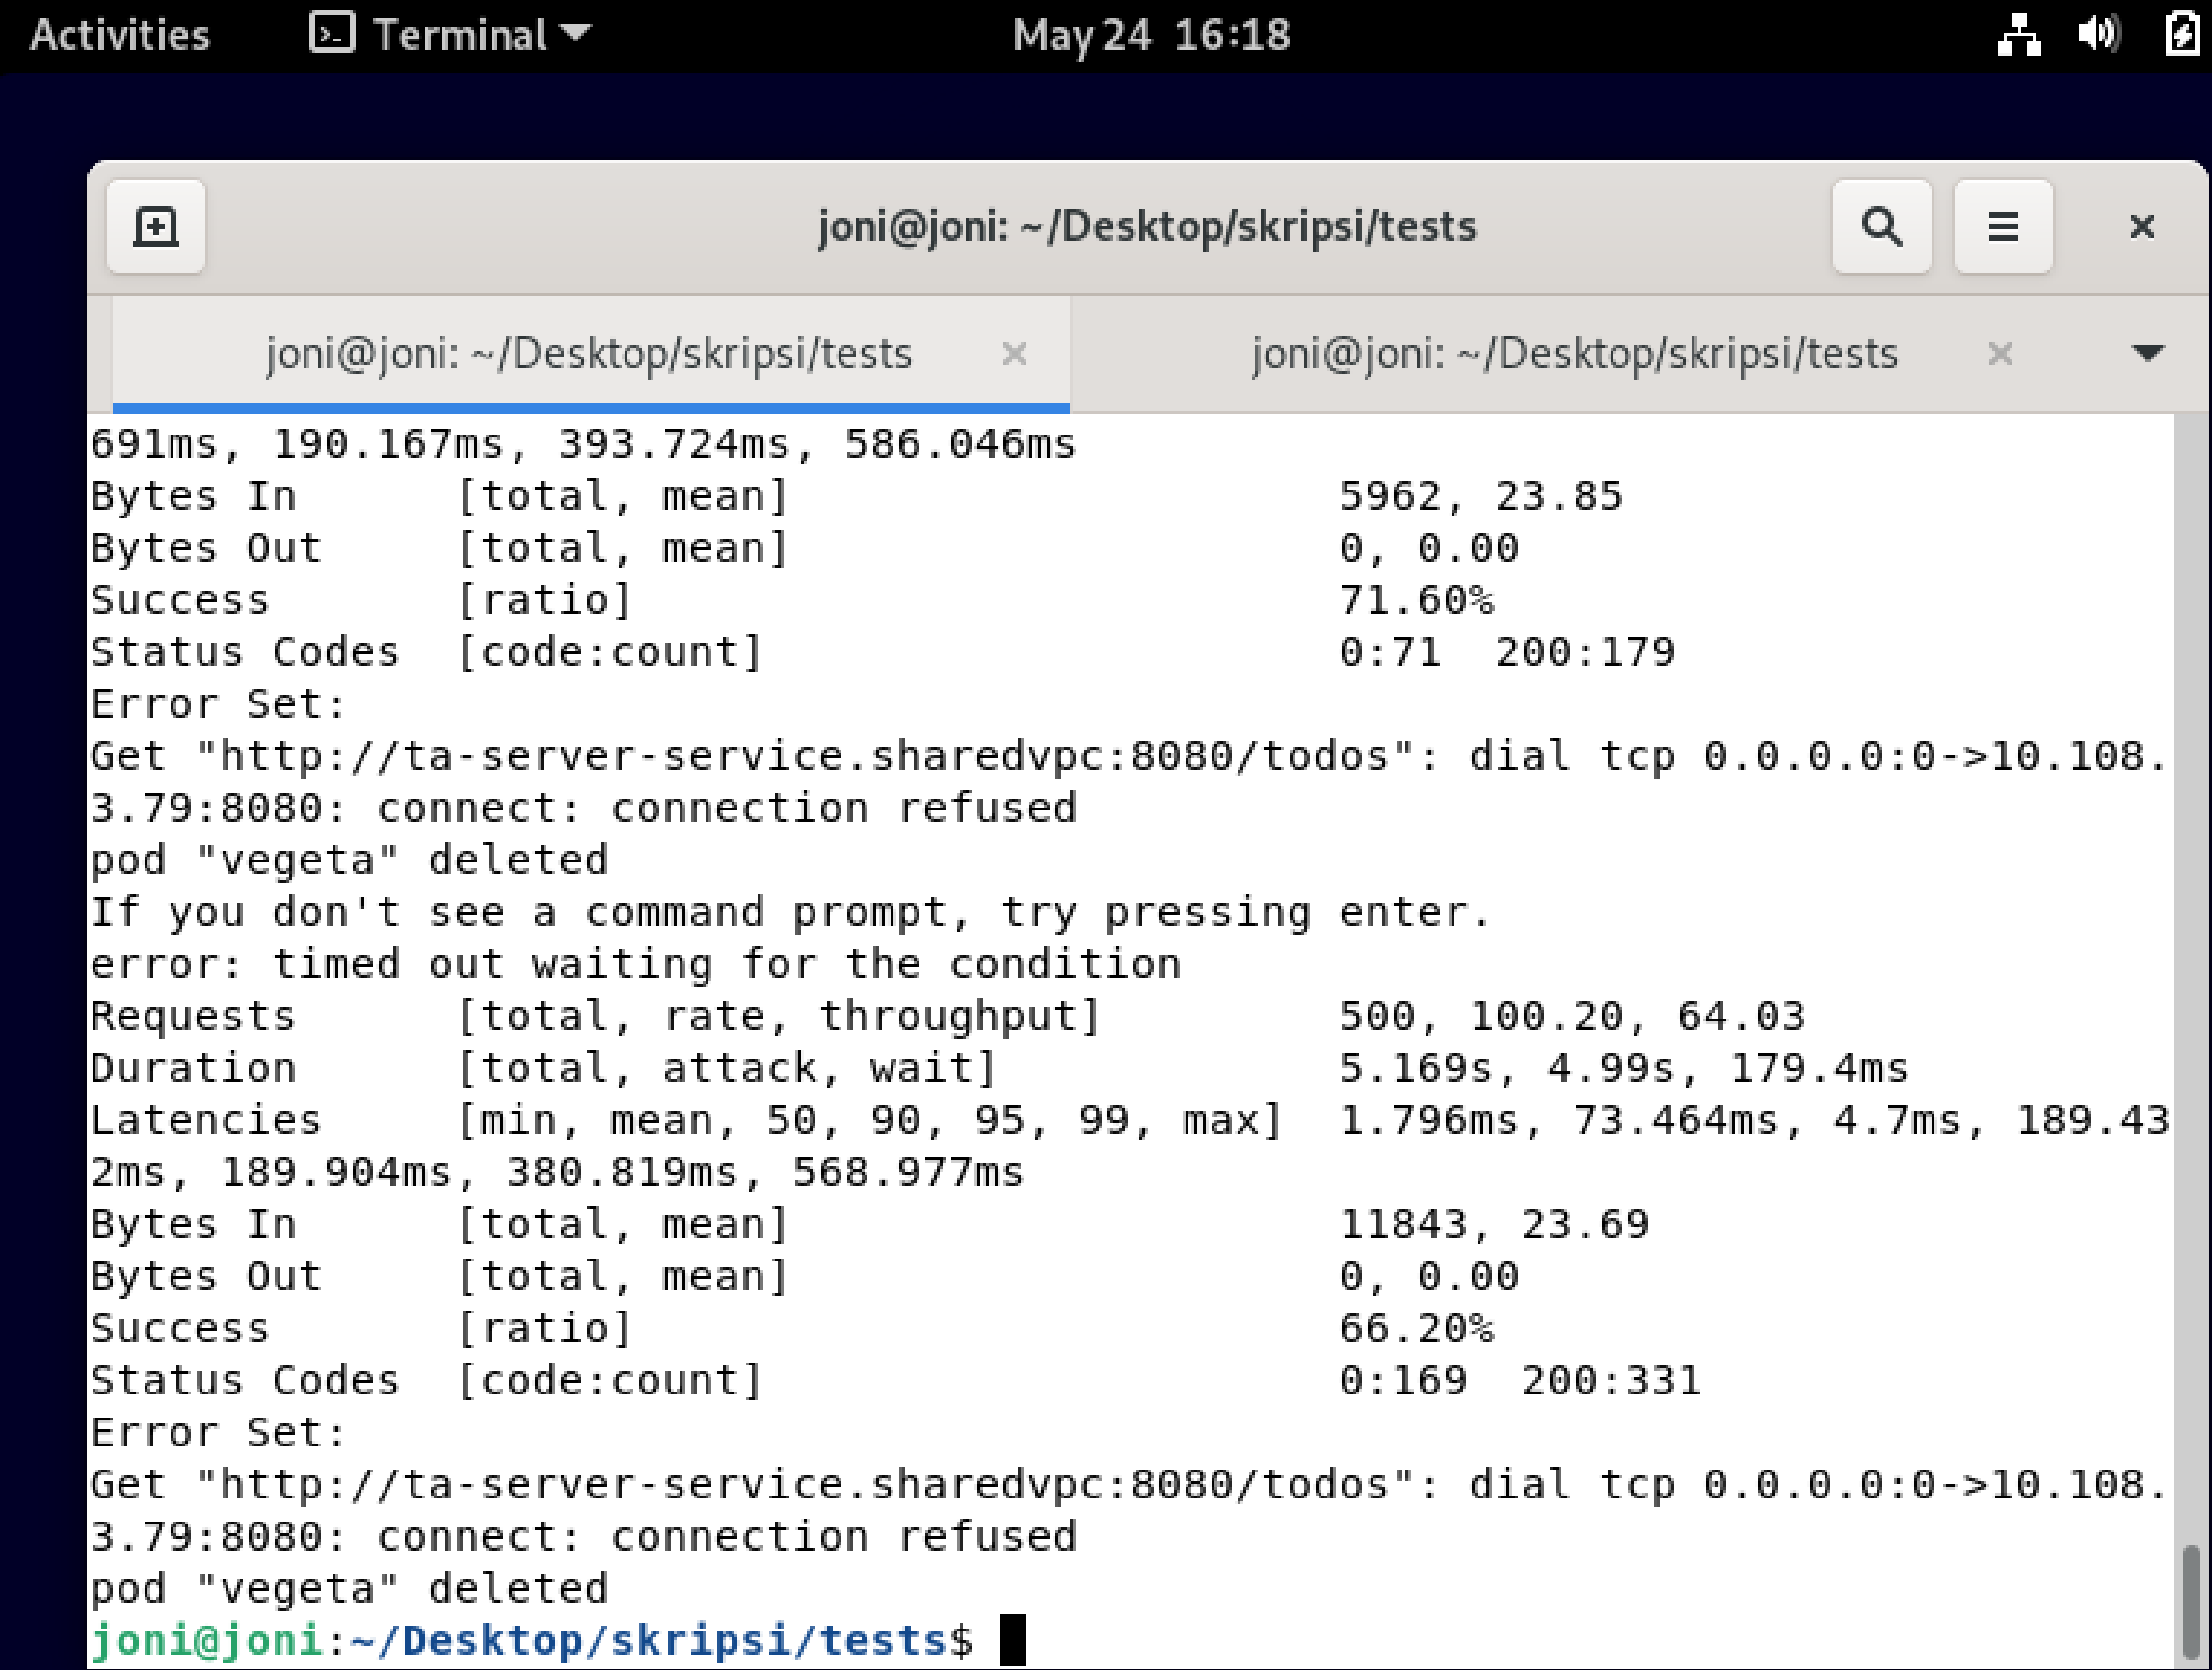
\includegraphics[width=1\textwidth]{assets/pics/error-code-0.png}
	\caption{Testing report with HTTP code 0 connection refused response.}
	\label{pic:error-code-0}
\end{figure}
\begin{figure}
	\centering
	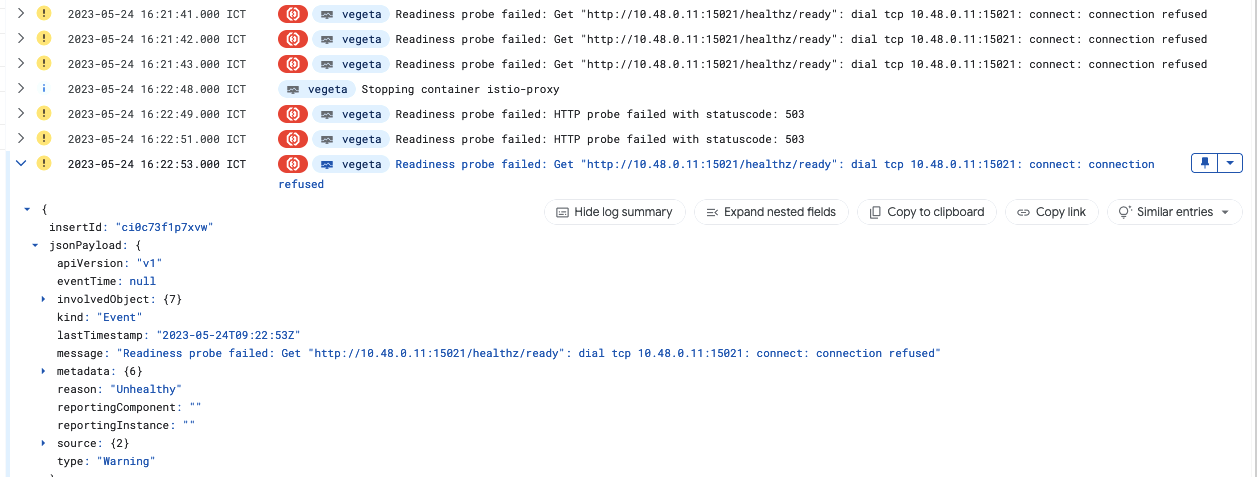
\includegraphics[width=1\textwidth]{assets/pics/readiness-probe-fail.png}
	\caption{Pod logs showing readiness probe fail.}
	\label{pic:readiness-probe-fail}
\end{figure}

There is also a discrepancy between the cluster's success ratio on Istio / ASM, where southeast-asia's has at least 2 times higher success ratio than its australia counterpart. As there are virtually no differences between the cluster's methods, this is perhaps an issue on the Google Cloud Platform's part, whether intended or not.


\begin{table}[h]
\centering
\caption{Multi-Cluster Reliability Test Results}

\begin{tabular}{|c|c|c|c|}
\hline

% \textbf{Method} & \textbf{Location} & \textbf{RPS} & \multicolumn{3}{c|}{\textbf{Latency (ms)}} & \textbf{Success Ratio} \\ \cline{4-6}
%  &  &  & \textbf{Min} & \textbf{Mean} & \textbf{Max} &  \\ \hline

\textbf{Method} & \textbf{Location} & \textbf{RPS} & \textbf{Success Ratio} \\ \hline
% TC 1 RES

%  & & 10 & 2.841179 & 3.687702 & 7.261602 & 100.00\% \\ \cline{3-7}
%  & southeast-asia & 50 & 2.48722 & 3.142731 & 6.367496 & 100.00\% \\ \cline{3-7}
% MCS with & & 100 & 3.835657 & 4.369947 & 8.858507 & 100.00\% \\ \cline{2-7}
% MCI & & 10 & 3.560003 & 4.743905 & 8.014017 & 100.00\% \\ \cline{3-7}
%  & australia & 50 & 3.938387 & 5.050108 & 10.318062 & 100.00\% \\ \cline{3-7}
%  & & 100 & 3.426384 & 4.202816 & 13.548108 & 100.00\% \\ \hline
%  & & 10 & 1.782431 & 3.627414 & 52.527168 & 40.00\% \\ \cline{3-7}
%  & southeast-asia & 50 & 1.511889 & 3.252973 & 33.364391 & 73.20\% \\ \cline{3-7}
% Istio / & & 100 & 1.48613 & 2.866272 & 33.372959 & 71.60\% \\ \cline{2-7}
% ASM & & 10 & 1.804273 & 29.992081 & 127.820017 & 32.00\% \\ \cline{3-7}
%  & australia & 50 & 1.721937 & 9.974838 & 96.424287 & 41.20\% \\ \cline{3-7}
%  & & 100 & 1.688115 & 5.778561 & 104.033348 & 31.40\% \\ \hline

% ALL TC RES
%  & & 10 & 2.841 & 3.836 & 8.219 & 100.00\% \\ \cline{3-7}
%  & southeast-asia & 50 & 2.487 & 3.657 & 8.992 & 100.00\% \\ \cline{3-7}
% MCS with & & 100 & 2.434 & 3.96 & 14.286 & 100.00\% \\ \cline{2-7}
% MCI & & 10 & 3.56 & 4.723 & 8.819 & 100.00\% \\ \cline{3-7}
%  & australia & 50 & 3.261 & 4.366 & 10.318 & 100.00\% \\ \cline{3-7}
%  & & 100 & 3.178 & 4.097 & 14.572 & 100.00\% \\ \hline
%  & & 10 & 1.745 & 3.709 & 52.527 & 62.67\% \\ \cline{3-7}
%  & southeast-asia & 50 & 1.512 & 3.232 & 35.926 & 71.87\% \\ \cline{3-7}
% Istio / & & 100 & 1.426 & 2.912 & 44.033 & 71.93\% \\ \cline{2-7}
% ASM & & 10 & 1.783 & 32.38 & 127.82 & 33.33\% \\ \cline{3-7}
%  & australia & 50 & 1.696 & 10.959 & 114.222 & 34.67\% \\ \cline{3-7}
%  & & 100 & 1.453 & 7.383 & 289.035 & 30.07\% \\ \hline

% FIXED LB
%  & & 10 & 2.841 & 3.836 & 8.219 & 100.00\% \\ \cline{3-7}
%  & southeast-asia & 50 & 2.487 & 3.657 & 8.992 & 100.00\% \\ \cline{3-7}
% MCS with & & 100 & 2.434 & 3.96 & 14.286 & 100.00\% \\ \cline{2-7}
% MCI & & 10 & 3.56 & 4.723 & 8.819 & 100.00\% \\ \cline{3-7}
%  & australia & 50 & 3.261 & 4.366 & 10.318 & 100.00\% \\ \cline{3-7}
%  & & 100 & 3.178 & 4.097 & 14.572 & 100.00\% \\ \hline
%  & & 10 & 3.497 & 35.543 & 103.985 & 100.00\% \\ \cline{3-7}
%  & southeast-asia & 50 & 3.594 & 10.724 & 103.524 & 100.00\% \\ \cline{3-7}
% Istio / & & 100 & 3.158 & 6.52 & 293.551 & 100.00\% \\ \cline{2-7}
% ASM & & 10 & 3.509 & 4.42 & 58.857 & 100.00\% \\ \cline{3-7}
%  & australia & 50 & 2.967 & 3.868 & 10.506 & 100.00\% \\ \cline{3-7}
%  & & 100 & 2.789 & 7.735 & 291.411 & 100.00\% \\ \hline
 
%  & & 10 & 1.745 & 3.709 & 52.527 & 62.67\% \\ \cline{3-7}
%  & southeast-asia & 50 & 1.512 & 3.232 & 35.926 & 71.87\% \\ \cline{3-7}
% Istio / ASM & & 100 & 1.426 & 2.912 & 44.033 & 71.93\% \\ \cline{2-7}
% (Single Cluster) & & 10 & 1.783 & 32.38 & 127.82 & 33.33\% \\ \cline{3-7}
%  & australia & 50 & 1.696 & 10.959 & 114.222 & 34.67\% \\ \cline{3-7}
%  & & 100 & 1.453 & 7.383 & 289.035 & 30.07\% \\ \hline

 & & 10 & 100.00\% \\ \cline{3-4}
 & southeast-asia & 50 & 100.00\% \\ \cline{3-4}
MCS with & & 100 & 100.00\% \\ \cline{2-4}
MCI & & 10 & 100.00\% \\ \cline{3-4}
 & australia & 50 & 100.00\% \\ \cline{3-4}
 & & 100 & 100.00\% \\ \hline
 & & 10 & 100.00\% \\ \cline{3-4}
 & southeast-asia & 50 & 100.00\% \\ \cline{3-4}
Istio / & & 100 & 100.00\% \\ \cline{2-4}
ASM & & 10 & 100.00\% \\ \cline{3-4}
 & australia & 50 & 100.00\% \\ \cline{3-4}
 & & 100 & 100.00\% \\ \hline

\end{tabular}
\label{tab:reliability-multi-cluster-results}
\end{table}

In contrast to single-cluster performance, multi-cluster performance seems to have fixed the reliability issue of Istio / ASM, where it can withstand 100 requests per second without a single failure. At the same time, the MCS with MCI maintains its perfect response ratio.

In addition, the server inside of a MCS with MCI method is able to handle 10 requests per second without restarting and only needs server recovery for 50 requests per second and above. In contrast, the server inside the Istio / ASM method needed to restart even during the lowest request per second configuration. This implies that a single cluster Istio / ASM may not be the most suitable geo-distributed approach for production-level applications, as it is unable to handle pedestrian-level traffic without inducing downtime on the servers. Therefore, it appears that MCS with MCI is more reliable than Istio / ASM for a single cluster configuration. It is advisable for Istio / ASM adopters to maximize its reliability by deploying services to multiple clusters and enabling the failover feature. Furthermore, there seems to be a problem with the Istio / ASM approach, where the failover feature of locality load balancing won't work with clients without a Service resource. This results in only one cluster responding to all of the requests without utilizing the other clusters.

In conclusion, the geo-distributed Kubernetes architecture is an effective way to increase the reliability of web applications, as it provides a connected network of clusters that serves as a failover when a cluster is experiencing downtime. There are also performance benefits to this, which we will see in \autoref{sec:5-perf}.

% \end{minipage}
% \begin{minipage}{.45\textwidth}
% \centering
% \begin{tabular}{|c|c|}
% \hline
% \textbf{Metric} & \textbf{Value} \\ \hline
% Success Ratio & 71.60\% \\ \hline
% \end{tabular}
% \caption{Success Metrics}
% \label{tab:success}
% \end{minipage}

% \todo{Tulis penjelasan terkait \tab~\ref{table:sample} di sini. Jika Anda hanya menunjukkan data, pembaca tidak akan tahu apakah data tersebut berharga.}


\section{Performance}
\label{sec:5-perf}

Istio / ASM's results may seem to be better for the single cluster configuration, especially if you compare the minimum latencies of each configuration from each method. However, this is simply the result of requests not being sent, resulting in it having a latency of under 2 milliseconds.

By comparing the minimum, average, and maximum latency of both configurations, as shown in \autoref{tab:multi-cluster-performance-results}, it can be seen that MCS with MCI has lower latency overall. Another important observation is the latency deviation produced by the Istio / ASM approach, where it may fluctuate to just under 300 milliseconds. This is a 171\% to 4385\% increase compared to MCS with MCI with a much more stable percentage increase between 136\% to 255\%.

\begin{table}[h]
\begin{adjustwidth}{-2cm}{-2cm}
 % \centering\makebox[\textwidth]
%  \centering\makebox{\textwidth}{}
%  % \centerline
%  {\resizebox{1.5\textwidth}{!}{%
\centering
\caption{Multi-Cluster Performance Test Results}

\begin{tabular}{|c|c|c|c|c|c|c|c|c|c|c|c|}
\hline

% \textbf{Method} & \textbf{Location} & \textbf{RPS} & \multicolumn{3}{c|}{\textbf{Latency (ms)}} & \textbf{Success Ratio} \\ \cline{4-6}
 % &  &  & \textbf{Min} & \textbf{Mean} & \textbf{Max} &  \\ \hline

% & & & & & \multicolumn{2}{c|}{\textbf{MCS with MCI}} & \multicolumn{2}{c|}{\textbf{Istio / ASM}}\\ \cline{5-6}
% \textbf{Method} & \textbf{Location} & \textbf{Test} & \textbf{RPS} & \multicolumn{2}{c|}{\textbf{Latency (ms)}} & \\ \cline{5-6}
%  &  & \textbf{Case} &  & \textbf{50th} & \textbf{95th} \\ \hline

% & & & \multicolumn{4}{c|}{\textbf{Latency (ms)}} \\ \cline{4-7}
% \textbf{Location} & \textbf{Test} & \textbf{RPS} & \multicolumn{2}{c|}{\textbf{50th}} & \multicolumn{2}{c|}{\textbf{95th}} \\ \cline{4-7}
% &  &  & \textbf{MCS} & \textbf{ASM} & \textbf{MCS} & \textbf{ASM} \\ \hline

% & & \multicolumn{10}{c|}{\textbf{Latency (ms)}} \\ \cline{3-12}
% \textbf{Location} & \textbf{RPS} & \multicolumn{2}{c|}{\textbf{50th}} & \multicolumn{2}{c|}{\textbf{95th}} & \multicolumn{2}{c|}{\textbf{Min}} & \multicolumn{2}{c|}{\textbf{Mean}}  & \multicolumn{2}{c|}{\textbf{Max}} \\ \cline{3-12}
% &  &  \textbf{MCS} & \textbf{ASM} & \textbf{MCS} & \textbf{ASM} & \textbf{MCS} & \textbf{ASM} & \textbf{MCS} & \textbf{ASM} & \textbf{MCS} & \textbf{ASM} \\ \hline

& & \multicolumn{10}{c|}{\textbf{Latency (ms)}} \\ \cline{3-12}
\textbf{Location} & \textbf{RPS} & \multicolumn{2}{c|}{\textbf{Min}} & \multicolumn{2}{c|}{\textbf{Median}} & \multicolumn{2}{c|}{\textbf{Mean}} & \multicolumn{2}{c|}{\textbf{95th}}  & \multicolumn{2}{c|}{\textbf{Max}} \\ \cline{3-12}
&  &  \textbf{MCS} & \textbf{ASM} & \textbf{MCS} & \textbf{ASM} & \textbf{MCS} & \textbf{ASM} & \textbf{MCS} & \textbf{ASM} & \textbf{MCS} & \textbf{ASM} \\ \hline

%  & southeast-asia & 1 & 10 & 3.37 & 5.593 \\ \cline{3-6}
%  & southeast-asia & 1 & 50 & 3.017 & 4.111 \\ \cline{3-6}
%  & southeast-asia & 1 & 100 & 4.286 & 4.861 \\ \cline{3-6}
%  & southeast-asia & 2 & 10 & 3.593 & 7.588 \\ \cline{3-6}
%  & southeast-asia & 2 & 50 & 3.322 & 4.033 \\ \cline{3-6}
%  & southeast-asia & 2 & 100 & 4.033 & 4.808 \\ \cline{3-6}
%  & southeast-asia & 3 & 10 & 3.47 & 5.068 \\ \cline{3-6}
%  & southeast-asia & 3 & 50 & 4.052 & 6.846 \\ \cline{3-6}
% MCS with & southeast-asia & 3 & 100 & 3.471 & 4.084 \\ \cline{2-6}
% MCI & australia & 1 & 10 & 4.492 & 6.693 \\ \cline{3-6}
%  & australia & 1 & 50 & 4.8 & 7.248 \\ \cline{3-6}
%  & australia & 1 & 100 & 3.958 & 5.943 \\ \cline{3-6}
%  & australia & 2 & 10 & 4.042 & 5.603 \\ \cline{3-6}
%  & australia & 2 & 50 & 3.799 & 5.355 \\ \cline{3-6}
%  & australia & 2 & 100 & 3.919 & 5.767 \\ \cline{3-6}
%  & australia & 3 & 10 & 4.745 & 6.946 \\ \cline{3-6}
%  & australia & 3 & 50 & 3.794 & 5.399 \\ \cline{3-6}
%  & australia & 3 & 100 & 3.797 & 5.156 \\ \hline
%  & southeast-asia & 1 & 10 & 4.2 & 4.826 \\ \cline{3-6}
%  & southeast-asia & 1 & 50 & 4.529 & 5.047 \\ \cline{3-6}
%  & southeast-asia & 1 & 100 & 4.26 & 96.766 \\ \cline{3-6}
%  & southeast-asia & 2 & 10 & 97.476 & 98.198 \\ \cline{3-6}
%  & southeast-asia & 2 & 50 & 4.464 & 97.65 \\ \cline{3-6}
%  & southeast-asia & 2 & 100 & 4.134 & 4.606 \\ \cline{3-6}
%  & southeast-asia & 3 & 10 & 4.42 & 4.908 \\ \cline{3-6}
%  & southeast-asia & 3 & 50 & 4.499 & 5.402 \\ \cline{3-6}
% Istio / & southeast-asia & 3 & 100 & 3.969 & 4.532 \\ \cline{2-6}
% ASM & australia & 1 & 10 & 3.951 & 4.686 \\ \cline{3-6}
%  & australia & 1 & 50 & 3.649 & 4.089 \\ \cline{3-6}
%  & australia & 1 & 100 & 3.582 & 4.074 \\ \cline{3-6}
%  & australia & 2 & 10 & 3.9 & 4.371 \\ \cline{3-6}
%  & australia & 2 & 50 & 3.977 & 4.471 \\ \cline{3-6}
%  & australia & 2 & 100 & 3.676 & 4.236 \\ \cline{3-6}
%  & australia & 3 & 10 & 3.902 & 4.554 \\ \cline{3-6}
%  & australia & 3 & 50 & 3.831 & 4.253 \\ \cline{3-6}
%  & australia & 3 & 100 & 3.621 & 96.294 \\ \hline

% southeast-asia & 1 & 10 & \textbf{3.37} & 4.2 & 5.593 & \textbf{4.826} \\ \cline{4-7}
% southeast-asia & 1 & 50 & \textbf{3.017} & 4.529 & \textbf{4.111} & 5.047 \\ \cline{4-7}
% southeast-asia & 1 & 100 & 4.286 & \textbf{4.26} & \textbf{4.861} & 96.766 \\ \cline{4-7}
% southeast-asia & 2 & 10 & \textbf{3.593} & 97.476 & \textbf{7.588} & 98.198 \\ \cline{4-7}
% southeast-asia & 2 & 50 & \textbf{3.322} & 4.464 & \textbf{4.033} & 97.65 \\ \cline{4-7}
% southeast-asia & 2 & 100 & \textbf{4.033} & 4.134 & 4.808 & \textbf{4.606} \\ \cline{4-7}
% southeast-asia & 3 & 10 & \textbf{3.47} & 4.42 & 5.068 & \textbf{4.908} \\ \cline{4-7}
% southeast-asia & 3 & 50 & \textbf{4.052} & 4.499 & 6.846 & \textbf{5.402} \\ \cline{4-7}
% southeast-asia & 3 & 100 & \textbf{3.471} & 3.969 & \textbf{4.084} & 4.532 \\ \cline{4-7}
% australia & 1 & 10 & 4.492 & \textbf{3.951} & 6.693 & \textbf{4.686} \\ \cline{4-7}
% australia & 1 & 50 & 4.8 & \textbf{3.649} & 7.248 & \textbf{4.089} \\ \cline{4-7}
% australia & 1 & 100 & 3.958 & \textbf{3.582} & 5.943 & \textbf{4.074} \\ \cline{4-7}
% australia & 2 & 10 & 4.042 & \textbf{3.9} & 5.603 & \textbf{4.371} \\ \cline{4-7}
% australia & 2 & 50 & \textbf{3.799} & 3.977 & 5.355 & \textbf{4.471} \\ \cline{4-7}
% australia & 2 & 100 & 3.919 & \textbf{3.676} & 5.767 & \textbf{4.236} \\ \cline{4-7}
% australia & 3 & 10 & 4.745 & \textbf{3.902} & 6.946 & \textbf{4.554} \\ \cline{4-7}
% australia & 3 & 50 & \textbf{3.794} & 3.831 & 5.399 & \textbf{4.253} \\ \cline{4-7}
% australia & 3 & 100 & 3.797 & \textbf{3.621} & \textbf{5.156} & 96.294 \\ \hline

% laporan v2.5
% southeast-asia & 10 & \textbf{3.37} & 4.826 & 5.593 & \textbf{4.826} &  &  &  &  &  &  \\ \cline{3-6}
% southeast-asia & 10 & \textbf{3.593} & 98.198 & \textbf{7.588} & 98.198 & \textbf{2.841} & 3.497 & \textbf{3.836} & 35.543 & \textbf{8.219} & 103.985 \\ \cline{3-6}
% southeast-asia & 10 & \textbf{3.47} & 4.908 & 5.068 & \textbf{4.908} &  &  &  &  &  &  \\ \hline
% southeast-asia & 50 & \textbf{3.017} & 5.047 & \textbf{4.111} & 5.047 &  &  &  &  &  &  \\ \cline{3-6}
% southeast-asia & 50 & \textbf{3.322} & 97.65 & \textbf{4.033} & 97.65 & \textbf{2.487} & 3.594 & \textbf{3.657} & 10.724 & \textbf{8.992} & 103.524 \\ \cline{3-6}
% southeast-asia & 50 & \textbf{4.052} & 5.402 & 6.846 & \textbf{5.402} &  &  &  &  &  &  \\ \hline
% southeast-asia & 100 & \textbf{4.286} & 96.766 & \textbf{4.861} & 96.766 &  &  &  &  &  &  \\ \cline{3-6}
% southeast-asia & 100 & \textbf{4.033} & 4.606 & 4.808 & \textbf{4.606} & \textbf{2.434} & 3.158 & \textbf{3.96} & 6.52 & \textbf{14.286} & 293.551 \\ \cline{3-6}
% southeast-asia & 100 & \textbf{3.471} & 4.532 & \textbf{4.084} & 4.532 &  &  &  &  &  &  \\ \hline
% australia & 10 & \textbf{4.492} & 4.686 & 6.693 & \textbf{4.686} &  &  &  &  &  &  \\ \cline{3-6}
% australia & 10 & \textbf{4.042} & 4.371 & 5.603 & \textbf{4.371} & 3.56 & \textbf{3.509} & 4.723 & \textbf{4.42} & \textbf{8.819} & 58.857 \\ \cline{3-6}
% australia & 10 & 4.745 & \textbf{4.554} & 6.946 & \textbf{4.554} &  &  &  &  &  &  \\ \hline
% australia & 50 & 4.8 & \textbf{4.089} & 7.248 & \textbf{4.089} &  &  &  &  &  &  \\ \cline{3-6}
% australia & 50 & \textbf{3.799} & 4.471 & 5.355 & \textbf{4.471} & 3.261 & \textbf{2.967} & 4.366 & \textbf{3.868} & \textbf{10.318} & 10.506 \\ \cline{3-6}
% australia & 50 & \textbf{3.794} & 4.253 & 5.399 & \textbf{4.253} &  &  &  &  &  &  \\ \hline
% australia & 100 & \textbf{3.958} & 4.074 & 5.943 & \textbf{4.074} &  &  &  &  &  &  \\ \cline{3-6}
% australia & 100 & \textbf{3.919} & 4.236 & 5.767 & \textbf{4.236} & 3.178 & \textbf{2.789} & \textbf{4.097} & 7.735 & \textbf{14.572} & 291.411 \\ \cline{3-6}
% australia & 100 & \textbf{3.797} & 96.294 & \textbf{5.156} & 96.294 &  &  &  &  &  &  \\ \hline

southeast-asia & 10 & \textbf{2.841} & 3.497 & \textbf{3.37} & 4.2 & \textbf{3.688} & 4.343 & 5.593 & \textbf{4.826} & \textbf{7.262} & 9.034 \\ \cline{3-12}
southeast-asia & 10 & \textbf{3.085} & 97.064 & \textbf{3.593} & 97.476 & \textbf{4.096} & 97.694 & \textbf{7.588} & 98.198 & \textbf{8.219} & 103.985 \\ \cline{3-12}
southeast-asia & 10 & \textbf{3.088} & 3.972 & \textbf{3.47} & 4.42 & \textbf{3.726} & 4.591 & 5.068 & \textbf{4.908} & \textbf{6.589} & 12.504 \\ \cline{3-12}
southeast-asia & 50 & \textbf{2.487} & 3.656 & \textbf{3.017} & 4.529 & \textbf{3.143} & 4.566 & \textbf{4.111} & 5.047 & \textbf{6.367} & 10.978 \\ \cline{3-12}
southeast-asia & 50 & \textbf{2.82} & 3.594 & \textbf{3.322} & 4.464 & \textbf{3.41} & 23.077 & \textbf{4.033} & 97.65 & \textbf{6.898} & 103.524 \\ \cline{3-12}
southeast-asia & 50 & \textbf{3.185} & 3.614 & \textbf{4.052} & 4.499 & \textbf{4.418} & 4.528 & 6.846 & \textbf{5.402} & \textbf{8.992} & 10.787 \\ \cline{3-12}
southeast-asia & 100 & 3.836 & \textbf{3.438} & 4.286 & \textbf{4.26} & \textbf{4.37} & 11.211 & \textbf{4.861} & 96.766 & \textbf{8.859} & 293.551 \\ \cline{3-12}
southeast-asia & 100 & \textbf{2.434} & 3.158 & \textbf{4.033} & 4.134 & \textbf{3.974} & 4.353 & 4.808 & \textbf{4.606} & \textbf{12.033} & 103.519 \\ \cline{3-12}
southeast-asia & 100 & \textbf{2.734} & 3.243 & \textbf{3.471} & 3.969 & \textbf{3.535} & 3.998 & \textbf{4.084} & 4.532 & 14.286 & \textbf{10.165} \\ \cline{3-12}
australia & 10 & \textbf{3.56} & 3.74 & 4.492 & \textbf{3.951} & \textbf{4.744} & 5.114 & 6.693 & \textbf{4.686} & \textbf{8.014} & 58.857 \\ \cline{3-12}
australia & 10 & 3.608 & \textbf{3.541} & 4.042 & \textbf{3.9} & 4.182 & \textbf{4.097} & 5.603 & \textbf{4.371} & \textbf{7.02} & 11.12 \\ \cline{3-12}
australia & 10 & 4.406 & \textbf{3.509} & 4.745 & \textbf{3.902} & 5.242 & \textbf{4.05} & 6.946 & \textbf{4.554} & \textbf{8.819} & 9.119 \\ \cline{3-12}
australia & 50 & 3.938 & \textbf{3.191} & 4.8 & \textbf{3.649} & 5.05 & \textbf{3.692} & 7.248 & \textbf{4.089} & 10.318 & \textbf{8.716} \\ \cline{3-12}
australia & 50 & 3.282 & \textbf{2.967} & \textbf{3.799} & 3.977 & \textbf{4.018} & 4.03 & 5.355 & \textbf{4.471} & \textbf{7.916} & 9.789 \\ \cline{3-12}
australia & 50 & \textbf{3.261} & 3.377 & \textbf{3.794} & 3.831 & 4.029 & \textbf{3.881} & 5.399 & \textbf{4.253} & \textbf{7.937} & 10.506 \\ \cline{3-12}
australia & 100 & 3.426 & \textbf{2.937} & 3.958 & \textbf{3.582} & 4.203 & \textbf{3.707} & 5.943 & \textbf{4.074} & \textbf{13.548} & 34.545 \\ \cline{3-12}
australia & 100 & 3.268 & \textbf{3.065} & 3.919 & \textbf{3.676} & 4.116 & \textbf{3.751} & 5.767 & \textbf{4.236} & 14.572 & \textbf{9.319} \\ \cline{3-12}
australia & 100 & 3.178 & \textbf{2.789} & 3.797 & \textbf{3.621} & \textbf{3.973} & 15.747 & \textbf{5.156} & 96.294 & \textbf{8.512} & 291.411 \\ \hline

\end{tabular}
% }}
\label{tab:multi-cluster-performance-results}
\end{adjustwidth}
\end{table}

In addition, both Istio / ASM and MCS with MCI approach correctly route traffic to the nearest cluster, as seen in \autoref{fig:5-sea-locality} and \autoref{fig:5-aus-locality}, where the server response, which contains the cluster name of the server that handled the request, corresponds to the cluster where the request originated from. This is a contrast to the study done by \citet{andrew-2023}, where it was stated that the Google Cloud Load Balancer didn't work correctly. It is to be noted that the MCS with MCI approach may simply be better integrated with Google Cloud Load Balancer compared to the DaemonSet resource used by \cite{andrew-2023}.

\begin{figure}
	\centering
	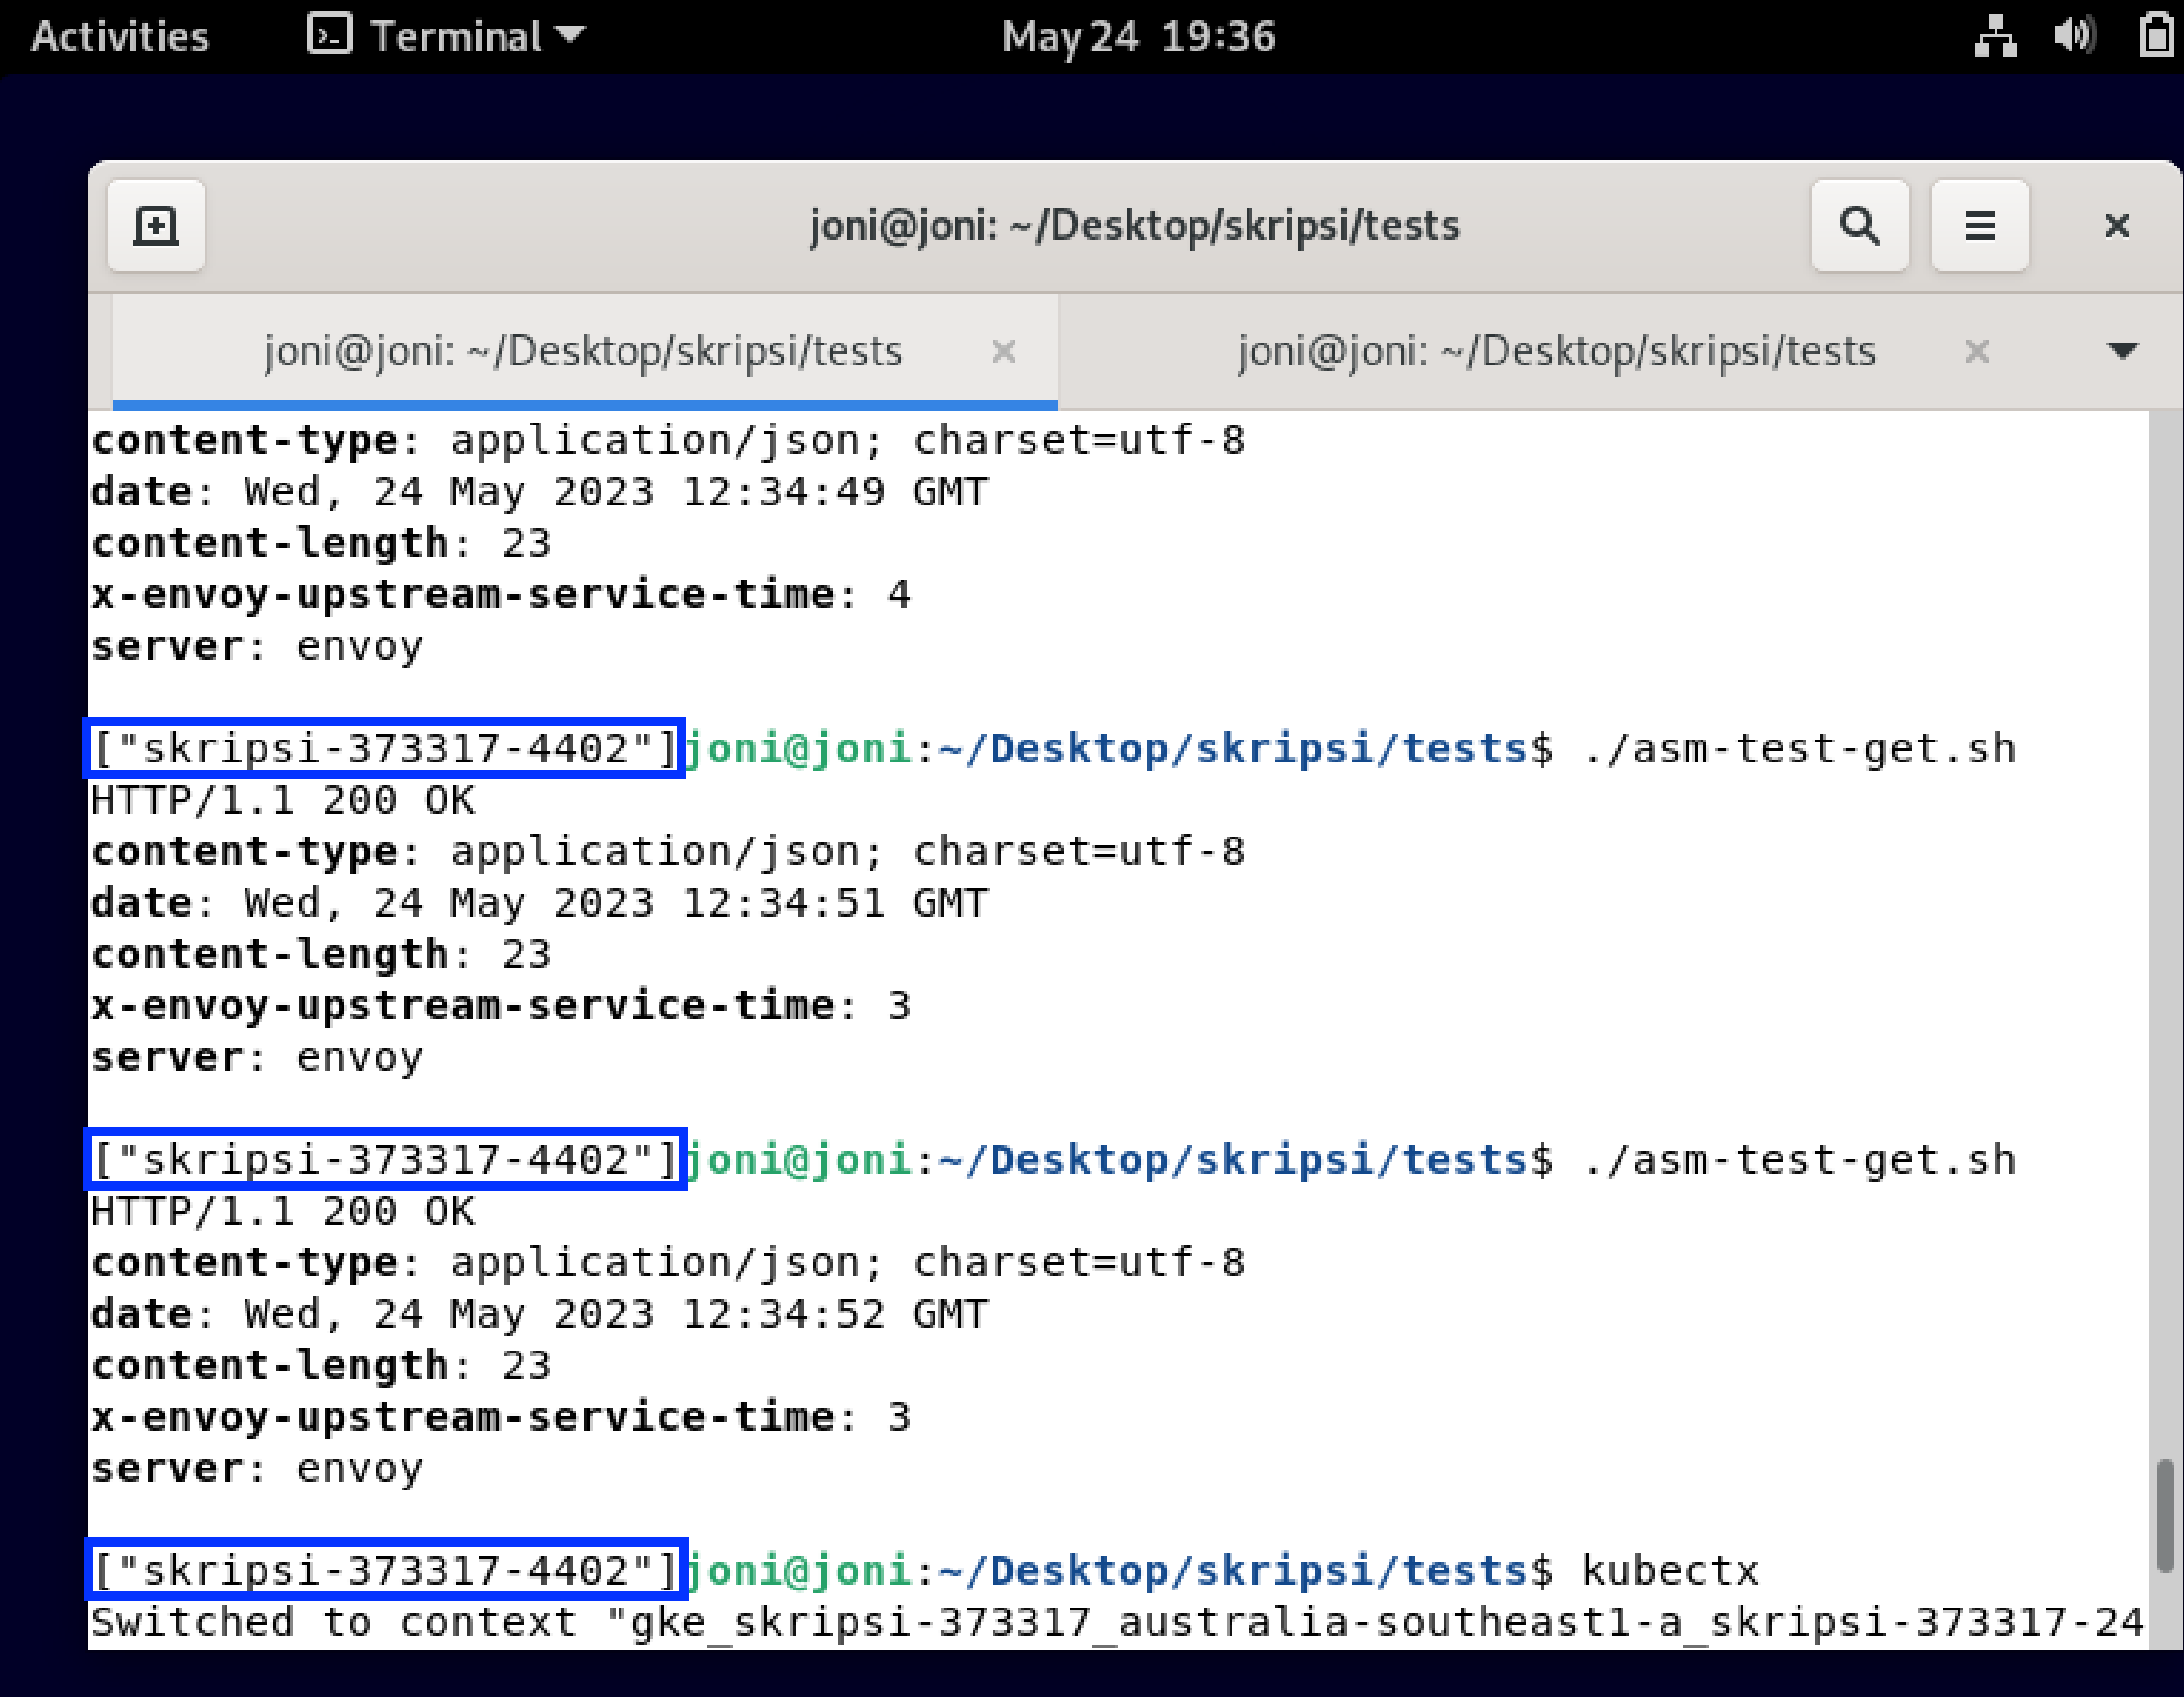
\includegraphics[width=1\textwidth]{assets/pics/5-sea-locality.png}
	\caption{Geo-aware routing from southeast-asia cluster.}
	\label{fig:5-sea-locality}
\end{figure}

\begin{figure}
	\centering
	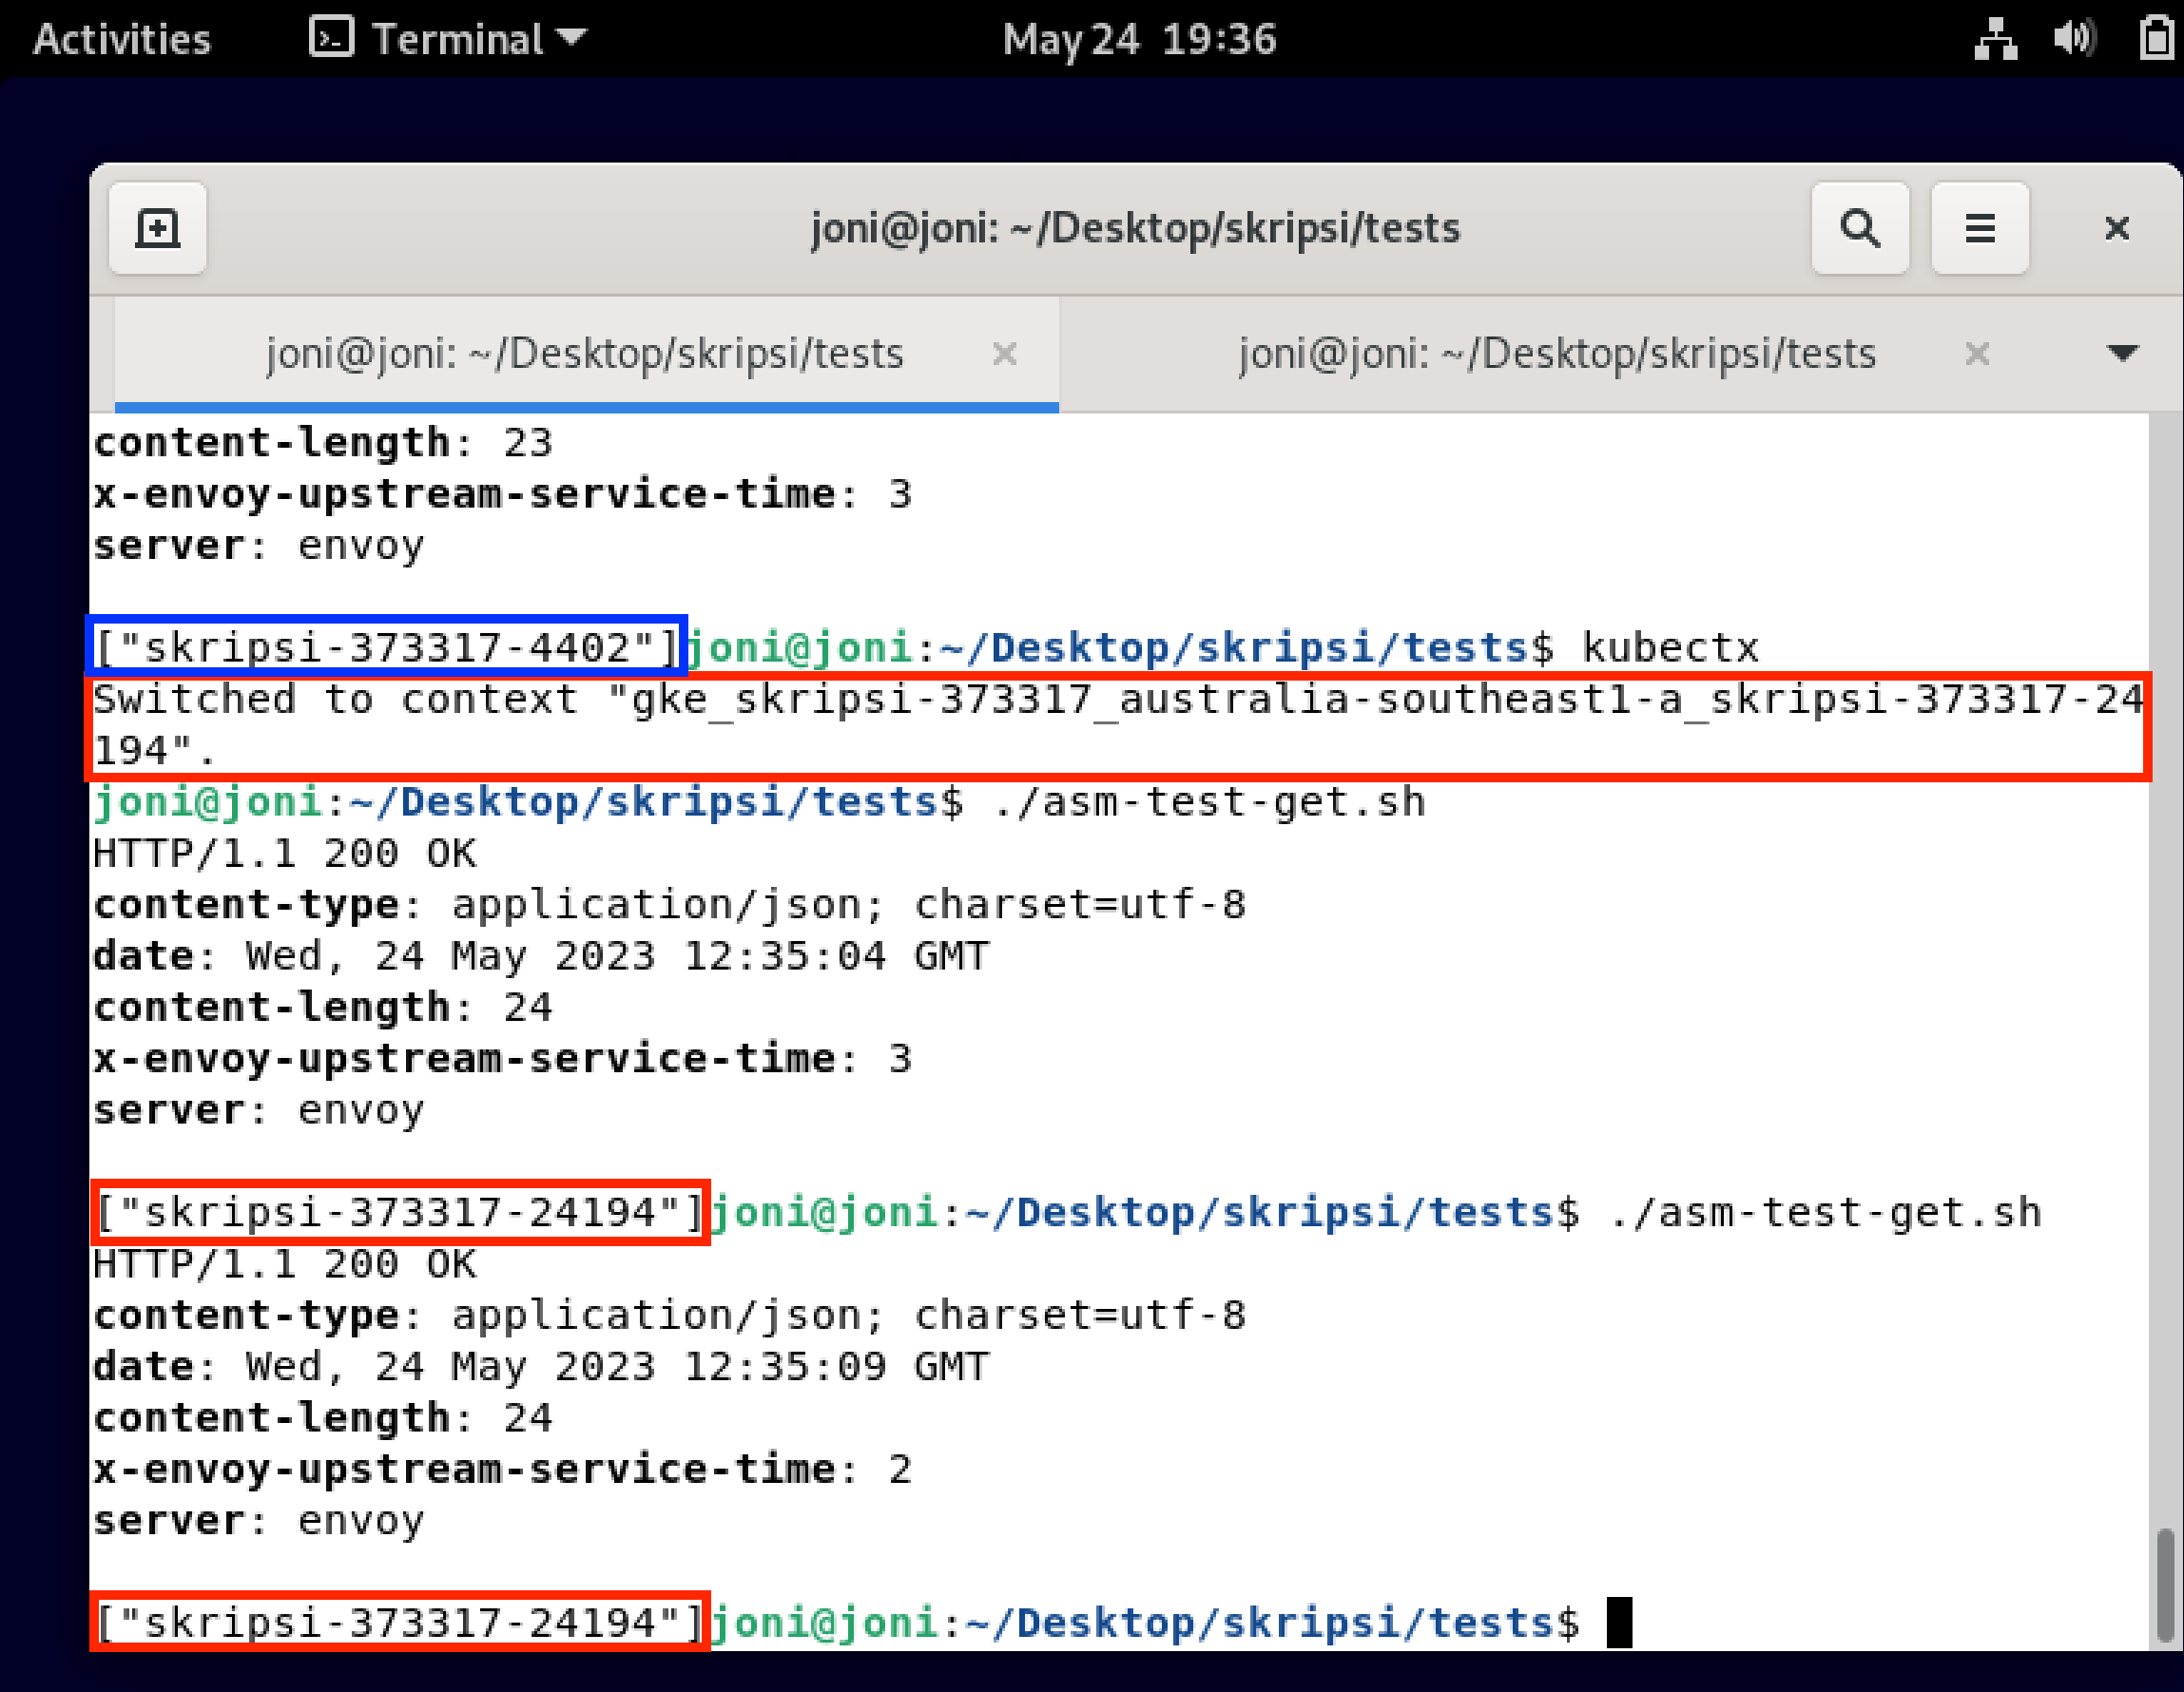
\includegraphics[width=1\textwidth]{assets/pics/5-aus-locality.png}
	\caption{Geo-aware routing from australia cluster.}
	\label{fig:5-aus-locality}
\end{figure}

Furthermore, the results from \autoref{tab:multi-cluster-performance-results} might indicate that MCS with MCI simply outperforms Istio / ASM, as it has a lower mean and lower maximum latency overall. However, it can be seen from \autoref{fig:latency-plot-mc-aus-2} and \autoref{fig:latency-plot-asm-aus-2} that the latency over time of Istio / ASM is comparable to MCI with MCS.

% \begin{table}[h]
% \centering
% \caption{Multi-Cluster Performance Test Results}

% \begin{tabular}{|c|c|c|c|c|c|c|c|}
% \hline


% & & \multicolumn{6}{c|}{\textbf{Latency (ms)}} \\ \cline{3-8}
% \textbf{Location} & \textbf{RPS} & \multicolumn{2}{c|}{\textbf{Min}} & \multicolumn{2}{c|}{\textbf{Mean}}  & \multicolumn{2}{c|}{\textbf{Max}} \\ \cline{3-8}
% &  & \textbf{MCS} & \textbf{ASM} & \textbf{MCS} & \textbf{ASM} & \textbf{MCS} & \textbf{ASM} \\ \hline


% southeast-asia & 10 & \textbf{2.841} & 3.497 & \textbf{3.836} & 35.543 & \textbf{8.219} & 103.985  \\ \cline{3-8}
% southeast-asia & 50 & \textbf{2.487} & 3.594 & \textbf{3.657} & 10.724 & \textbf{8.992} & 103.524  \\ \cline{3-8}
% southeast-asia & 100 & \textbf{2.434} & 3.158 & \textbf{3.96} & 6.52 & \textbf{14.286} & 293.551  \\ \cline{3-8}
% australia & 10 & 3.56 & \textbf{3.509} & 4.723 & \textbf{4.42} & \textbf{8.819} & 58.857 \\ \cline{3-8}
% australia & 50 & 3.261 & \textbf{2.967} & 4.366 & \textbf{3.868} & \textbf{10.318} & 10.506 \\ \cline{3-8}
% australia & 100 & 3.178 & \textbf{2.789} & \textbf{4.097} & 7.735 & \textbf{14.572} & 291.411  \\ \hline

% \end{tabular}
% \label{tab:mean-multi-cluster-results}
% \end{table}

\begin{figure}
	\centering
	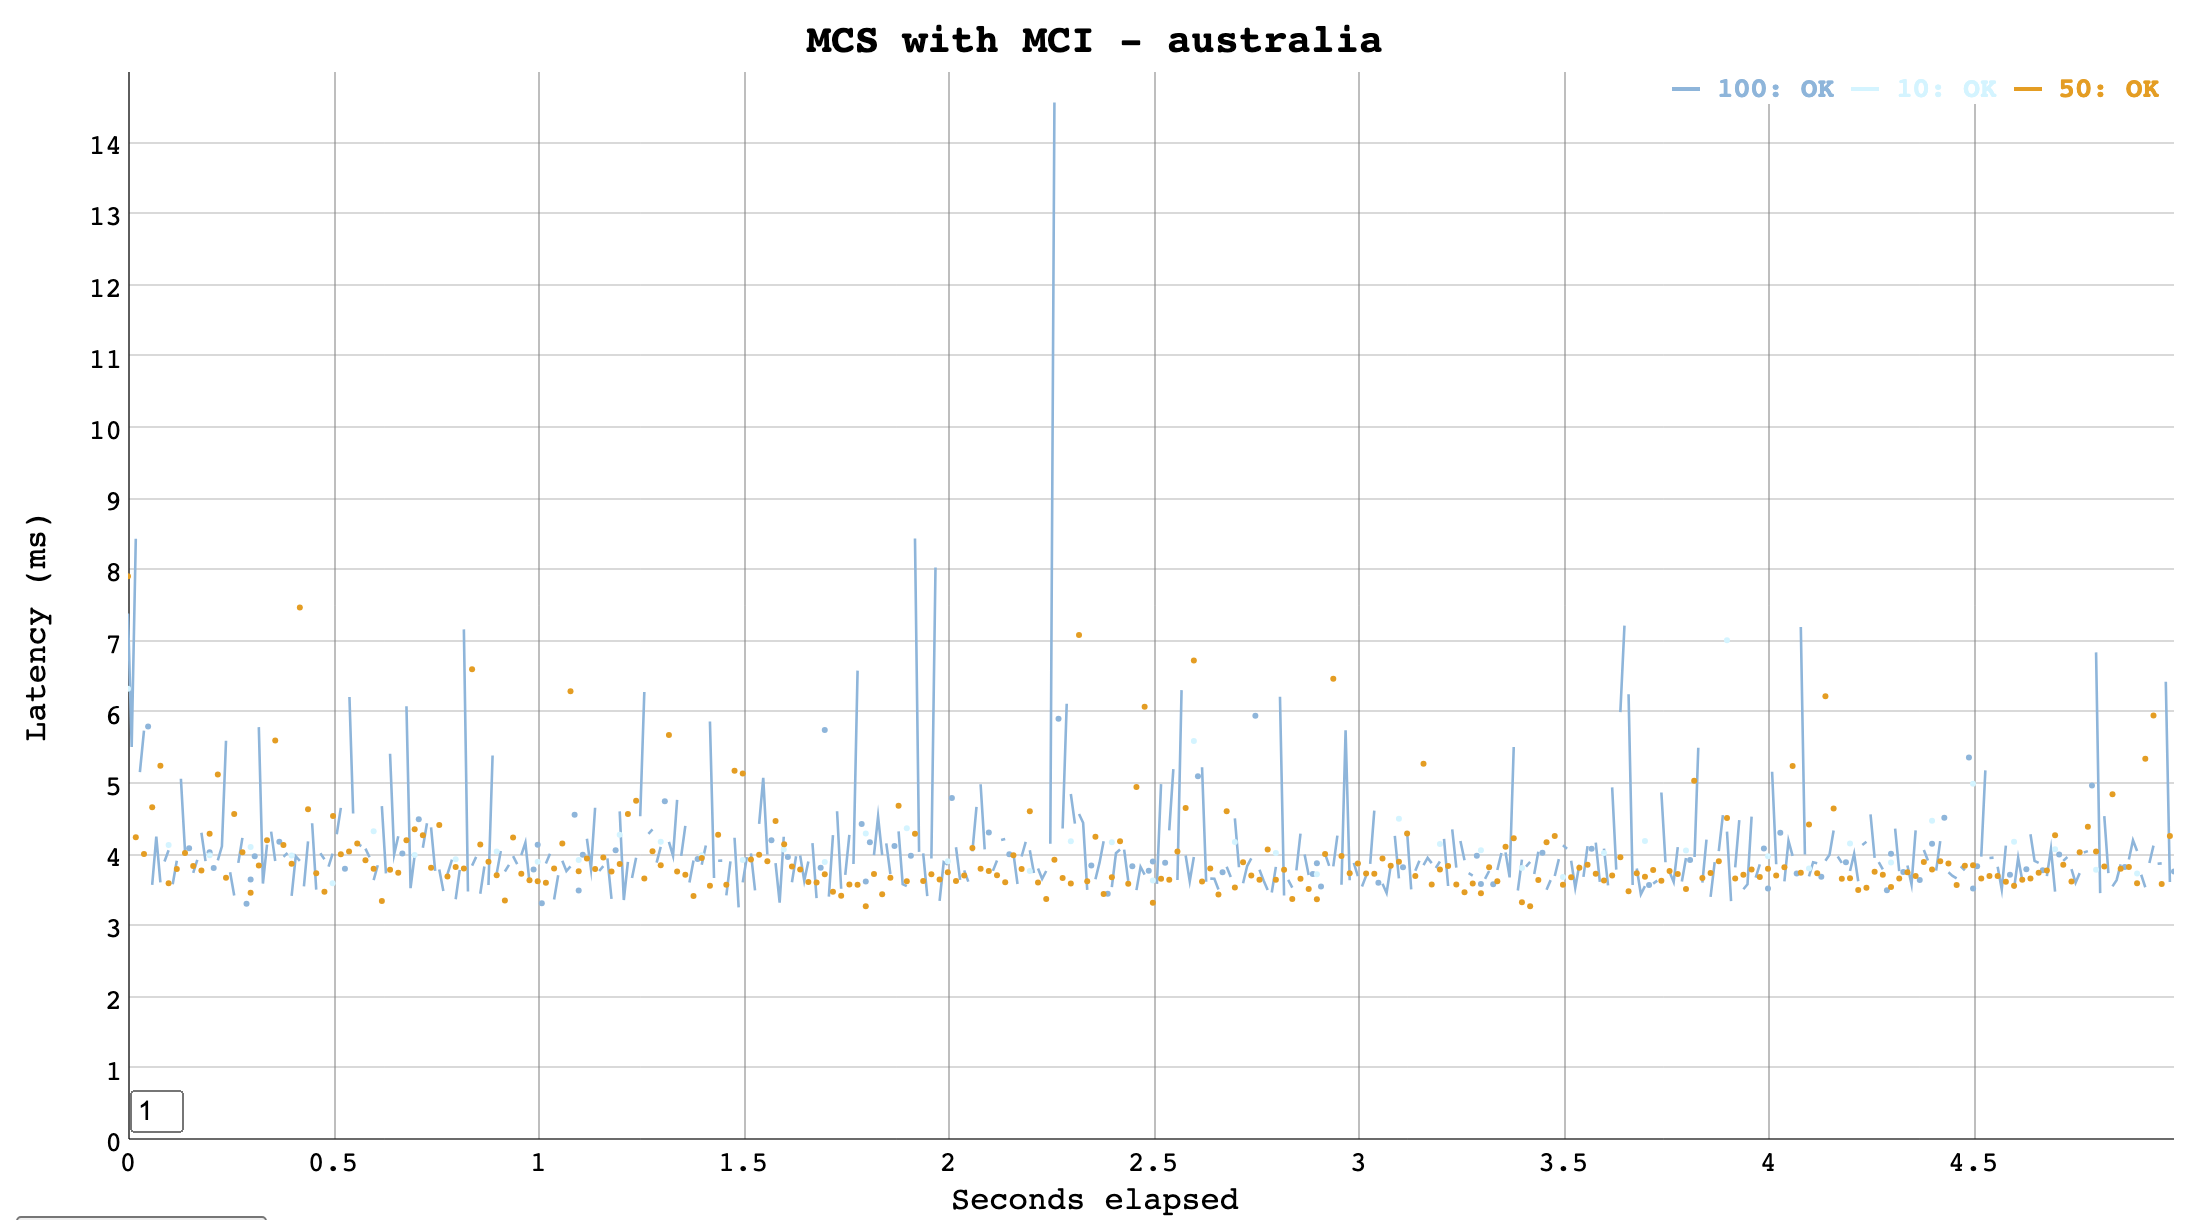
\includegraphics[width=1\textwidth]{assets/plots/mc-aus-2.png}
	\caption{Latency over time of MCS with MCI australia 3.}
	\label{fig:latency-plot-mc-aus-2}
\end{figure}

\begin{figure}
	\centering
	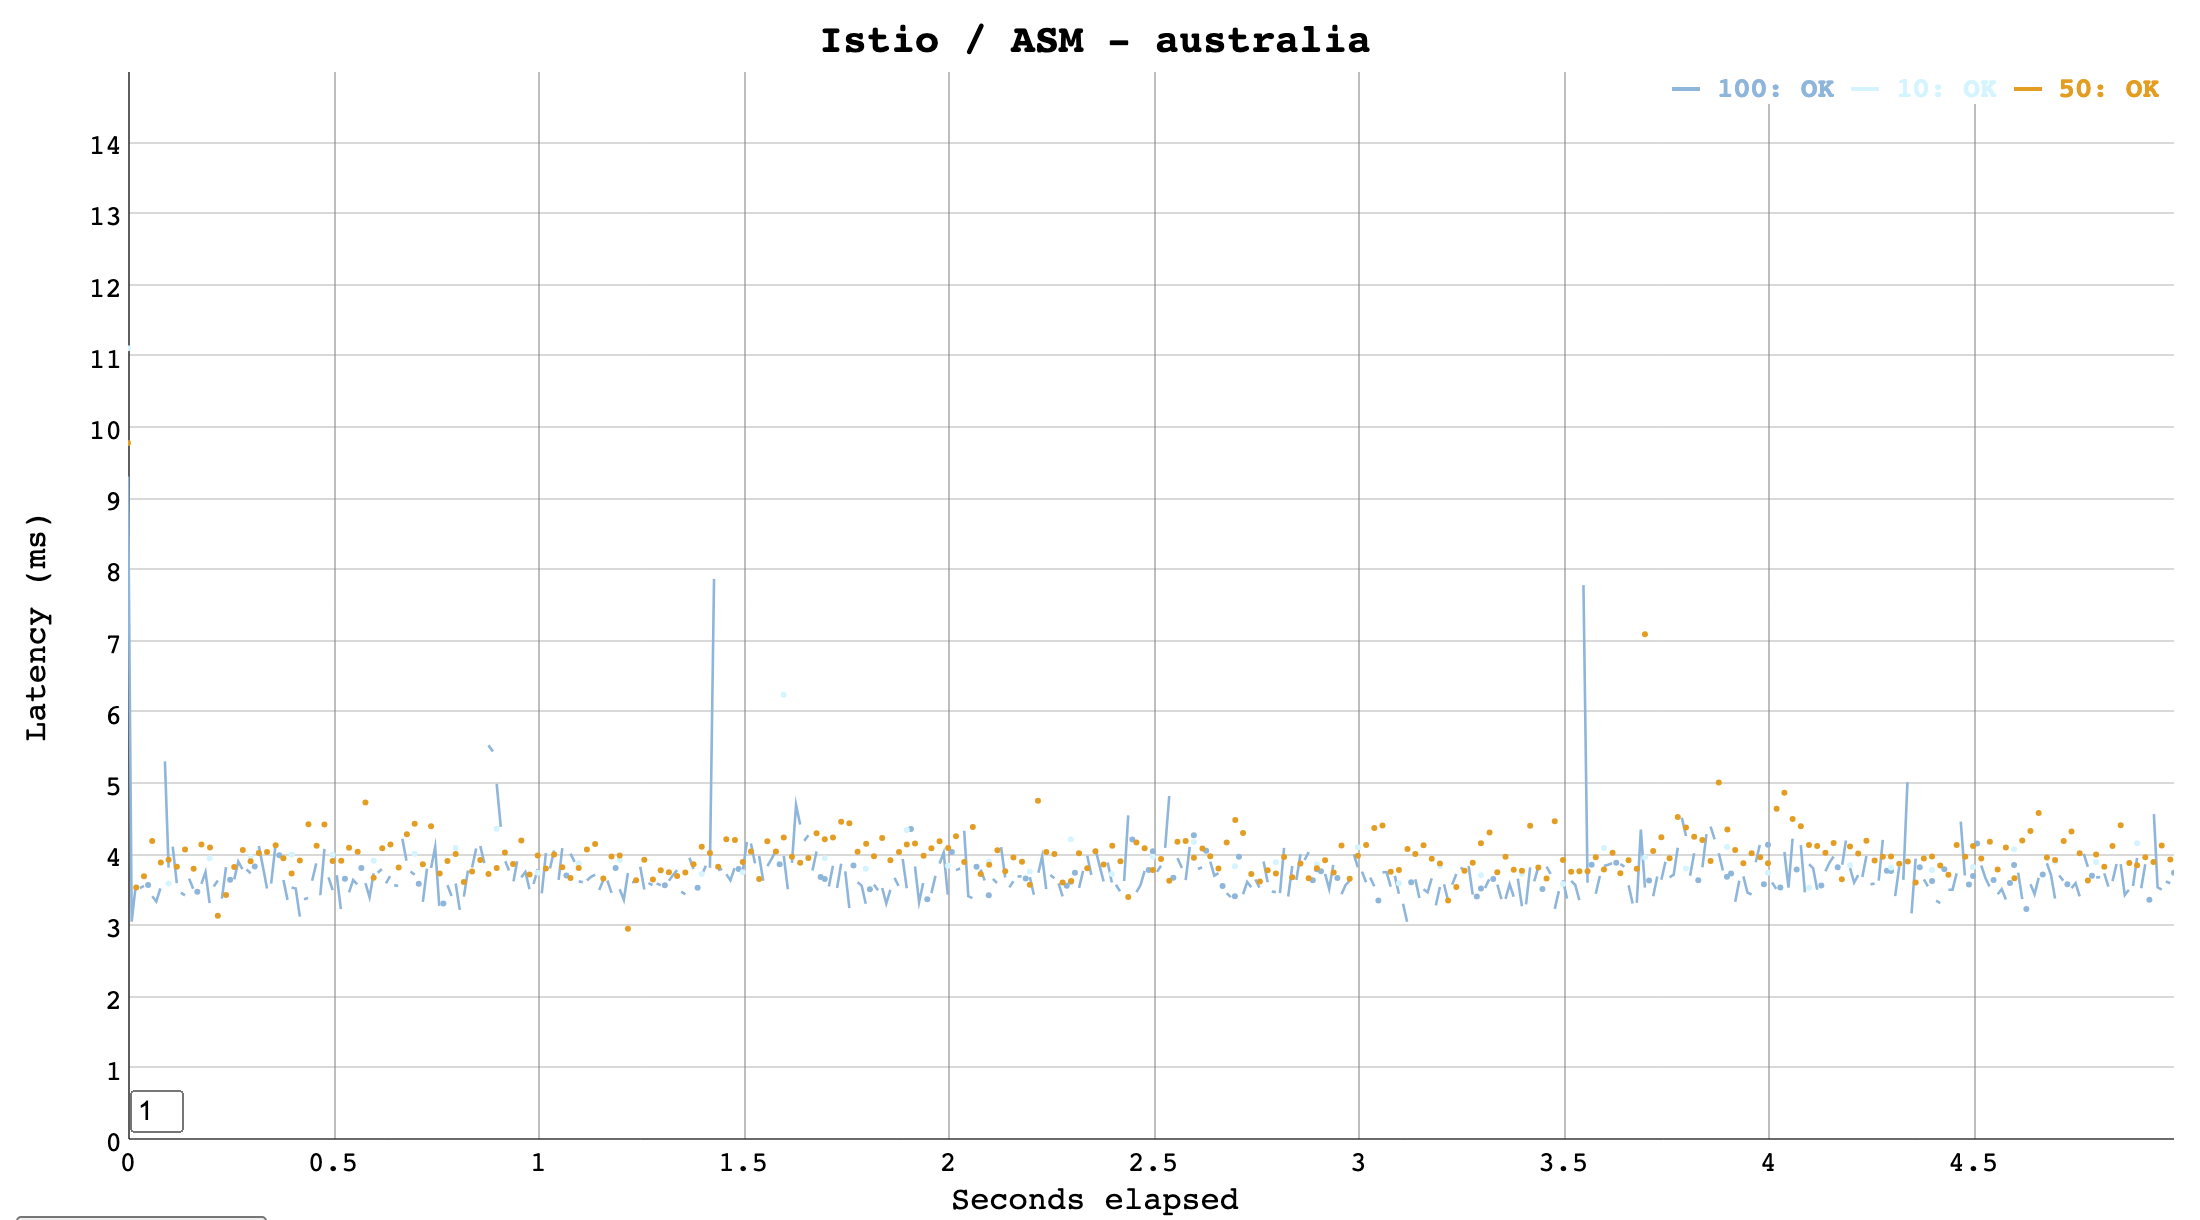
\includegraphics[width=1\textwidth]{assets/plots/asm-aus-2.png}
	\caption{Latency over time of Istio / ASM australia 2.}
	\label{fig:latency-plot-asm-aus-2}
\end{figure}

Further testing shows that the reason Istio / ASM method has a worse overall result is the occurrence of performance outliers, as seen in \autoref{fig:latency-plot-asm-sea-1} and  \autoref{fig:latency-plot-asm-aus-3}, the latency over time for the southeast-asia and australia region, respectively. These outliers produced responses with upwards of 300 milliseconds latency and indicate that the Istio / ASM method is prone to under-performance during high-traffic situations. This can be explained by the slow server recovery time shown in \autoref{tab:reliability-single-cluster-results}, where the failed responses must be redirected to a server with a nonoptimal geographic distance.

\begin{figure}
	\centering
	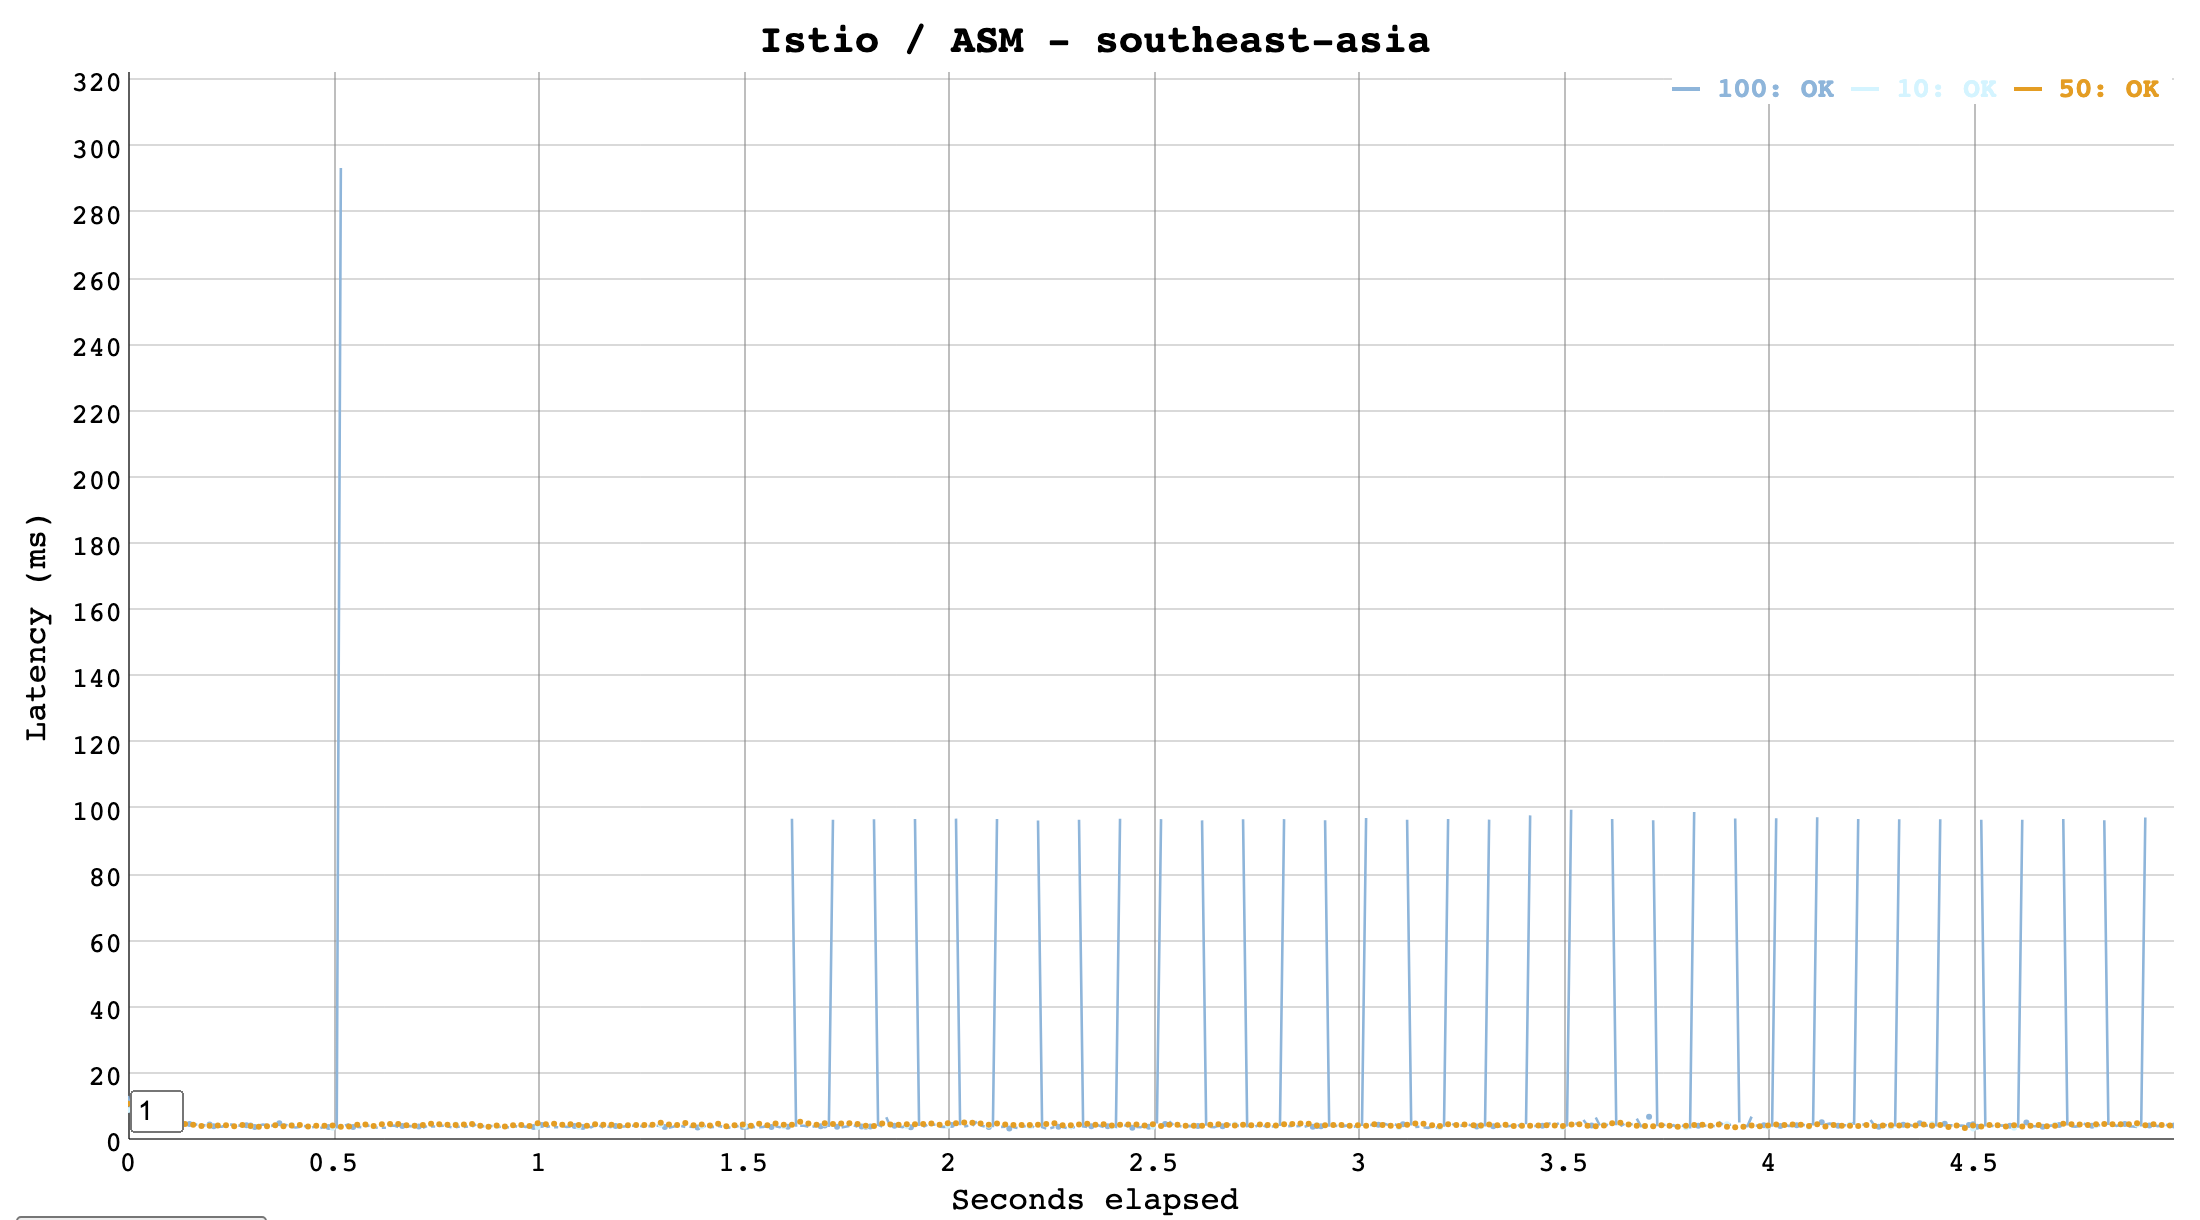
\includegraphics[width=1\textwidth]{assets/plots/asm-sea-1.png}
    \caption{Latency over time of Istio / ASM southeast-asia 1.}
	\label{fig:latency-plot-asm-sea-1}
\end{figure}

\begin{figure}
	\centering
	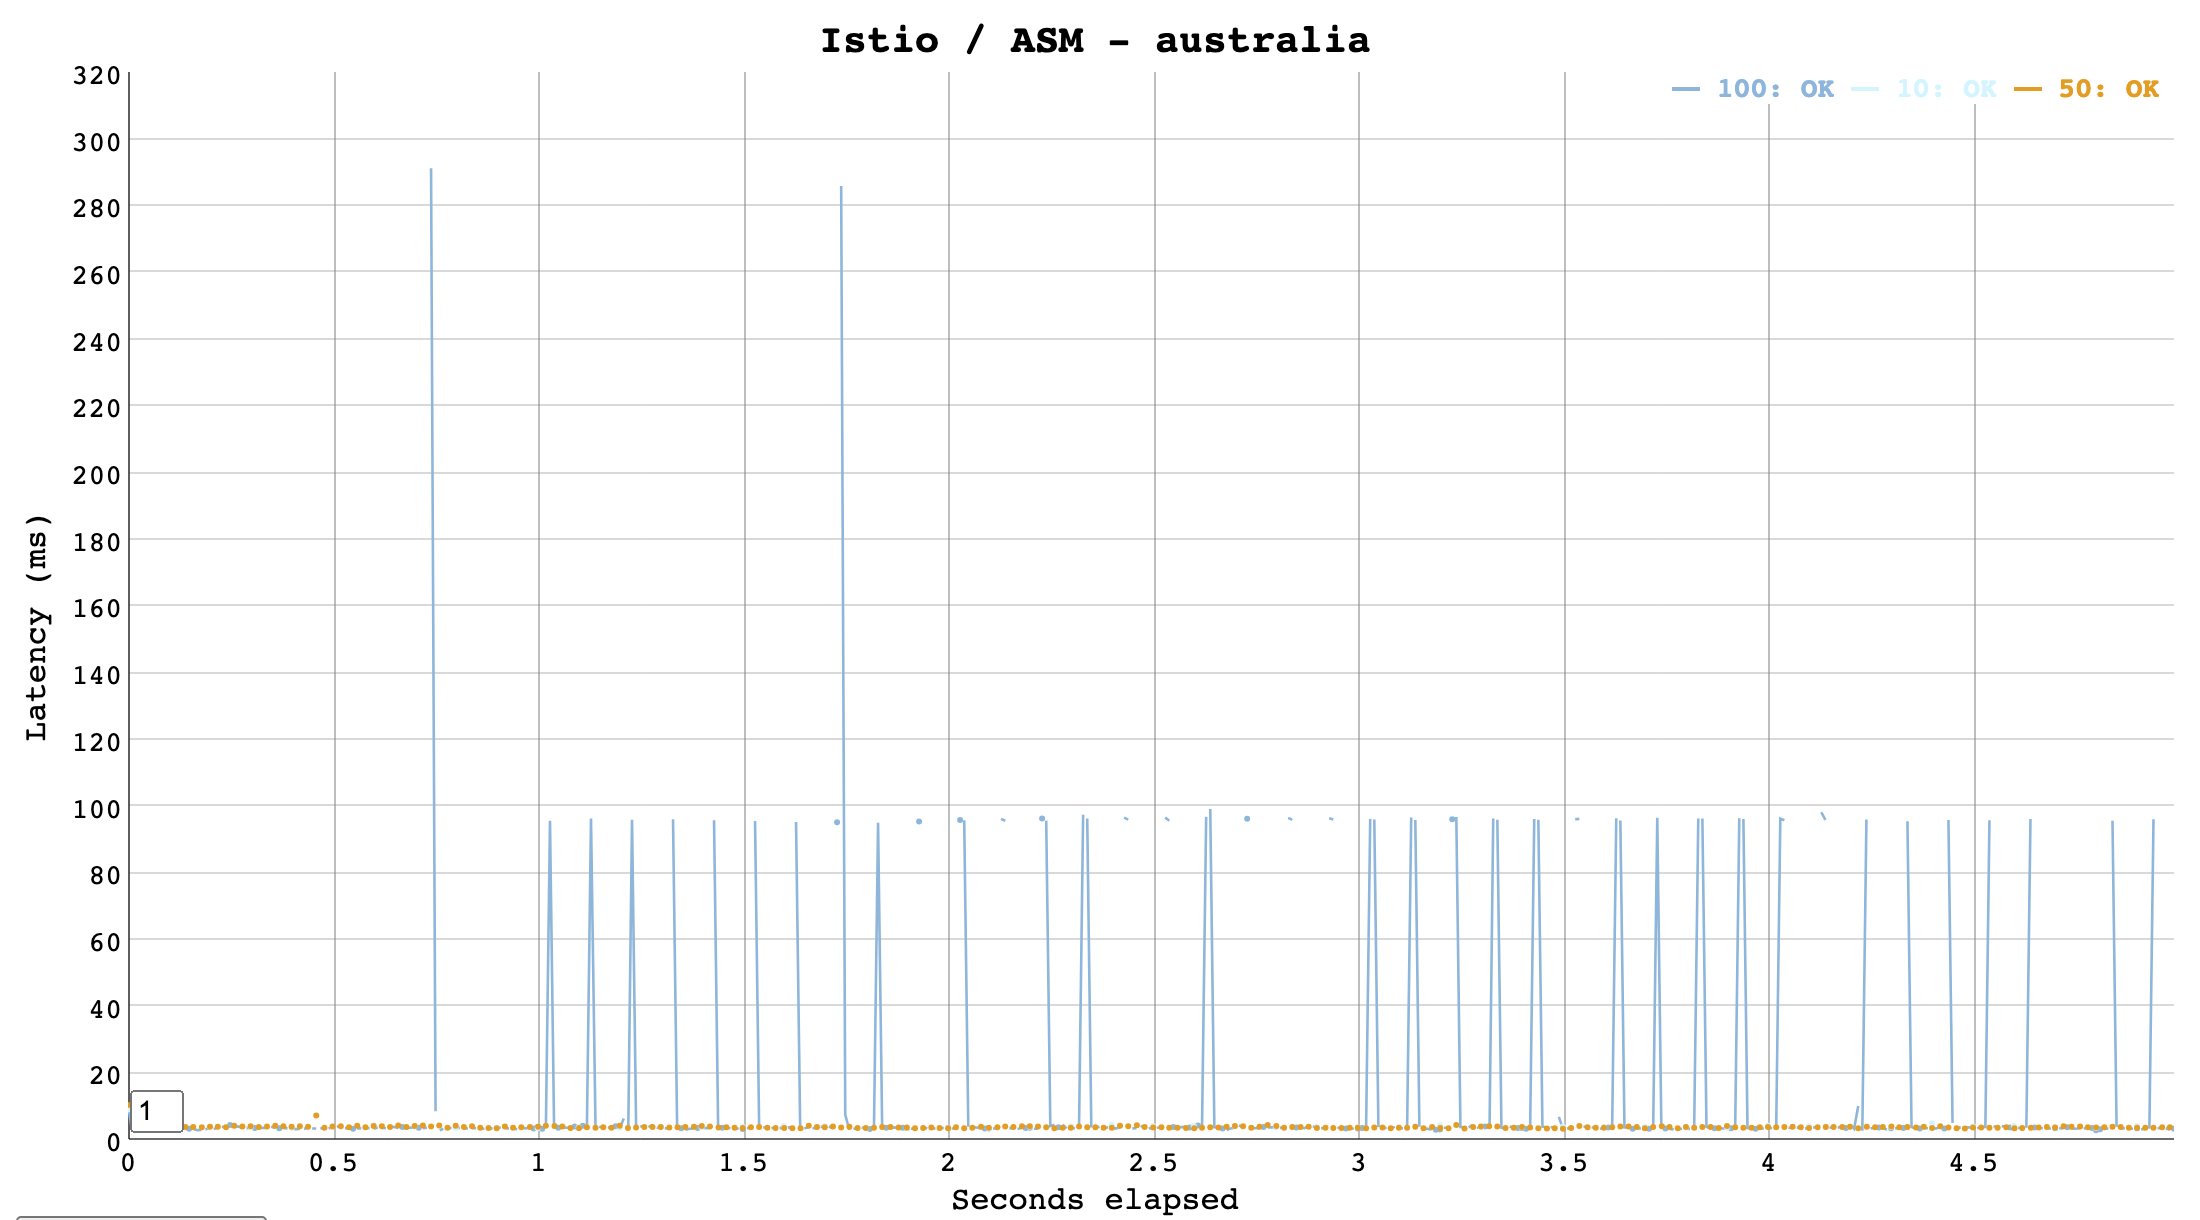
\includegraphics[width=1\textwidth]{assets/plots/asm-aus-3.png}
	\caption{Latency over time of Istio / ASM australia 3.}
	\label{fig:latency-plot-asm-aus-3}
\end{figure}

Conversely, test results from MCS with MCI as seen in \autoref{fig:latency-plot-mc-aus-1} and \autoref{fig:latency-plot-mc-sea-1} show its consistency as it is able to maintain its performance through multiple experiments. There hasn't been an occurrence where MCS with MCI takes longer than 15 milliseconds to respond. This can be explained by MCS with MCI's excellent single-cluster performance, as its server is able to recover from failure in a short amount of time. Furthermore, a single-cluster MCS with MCI outperforms a multi-cluster Istio / ASM configuration in overall latency with an equivalently flawless success ratio.

\begin{figure}
	\centering
	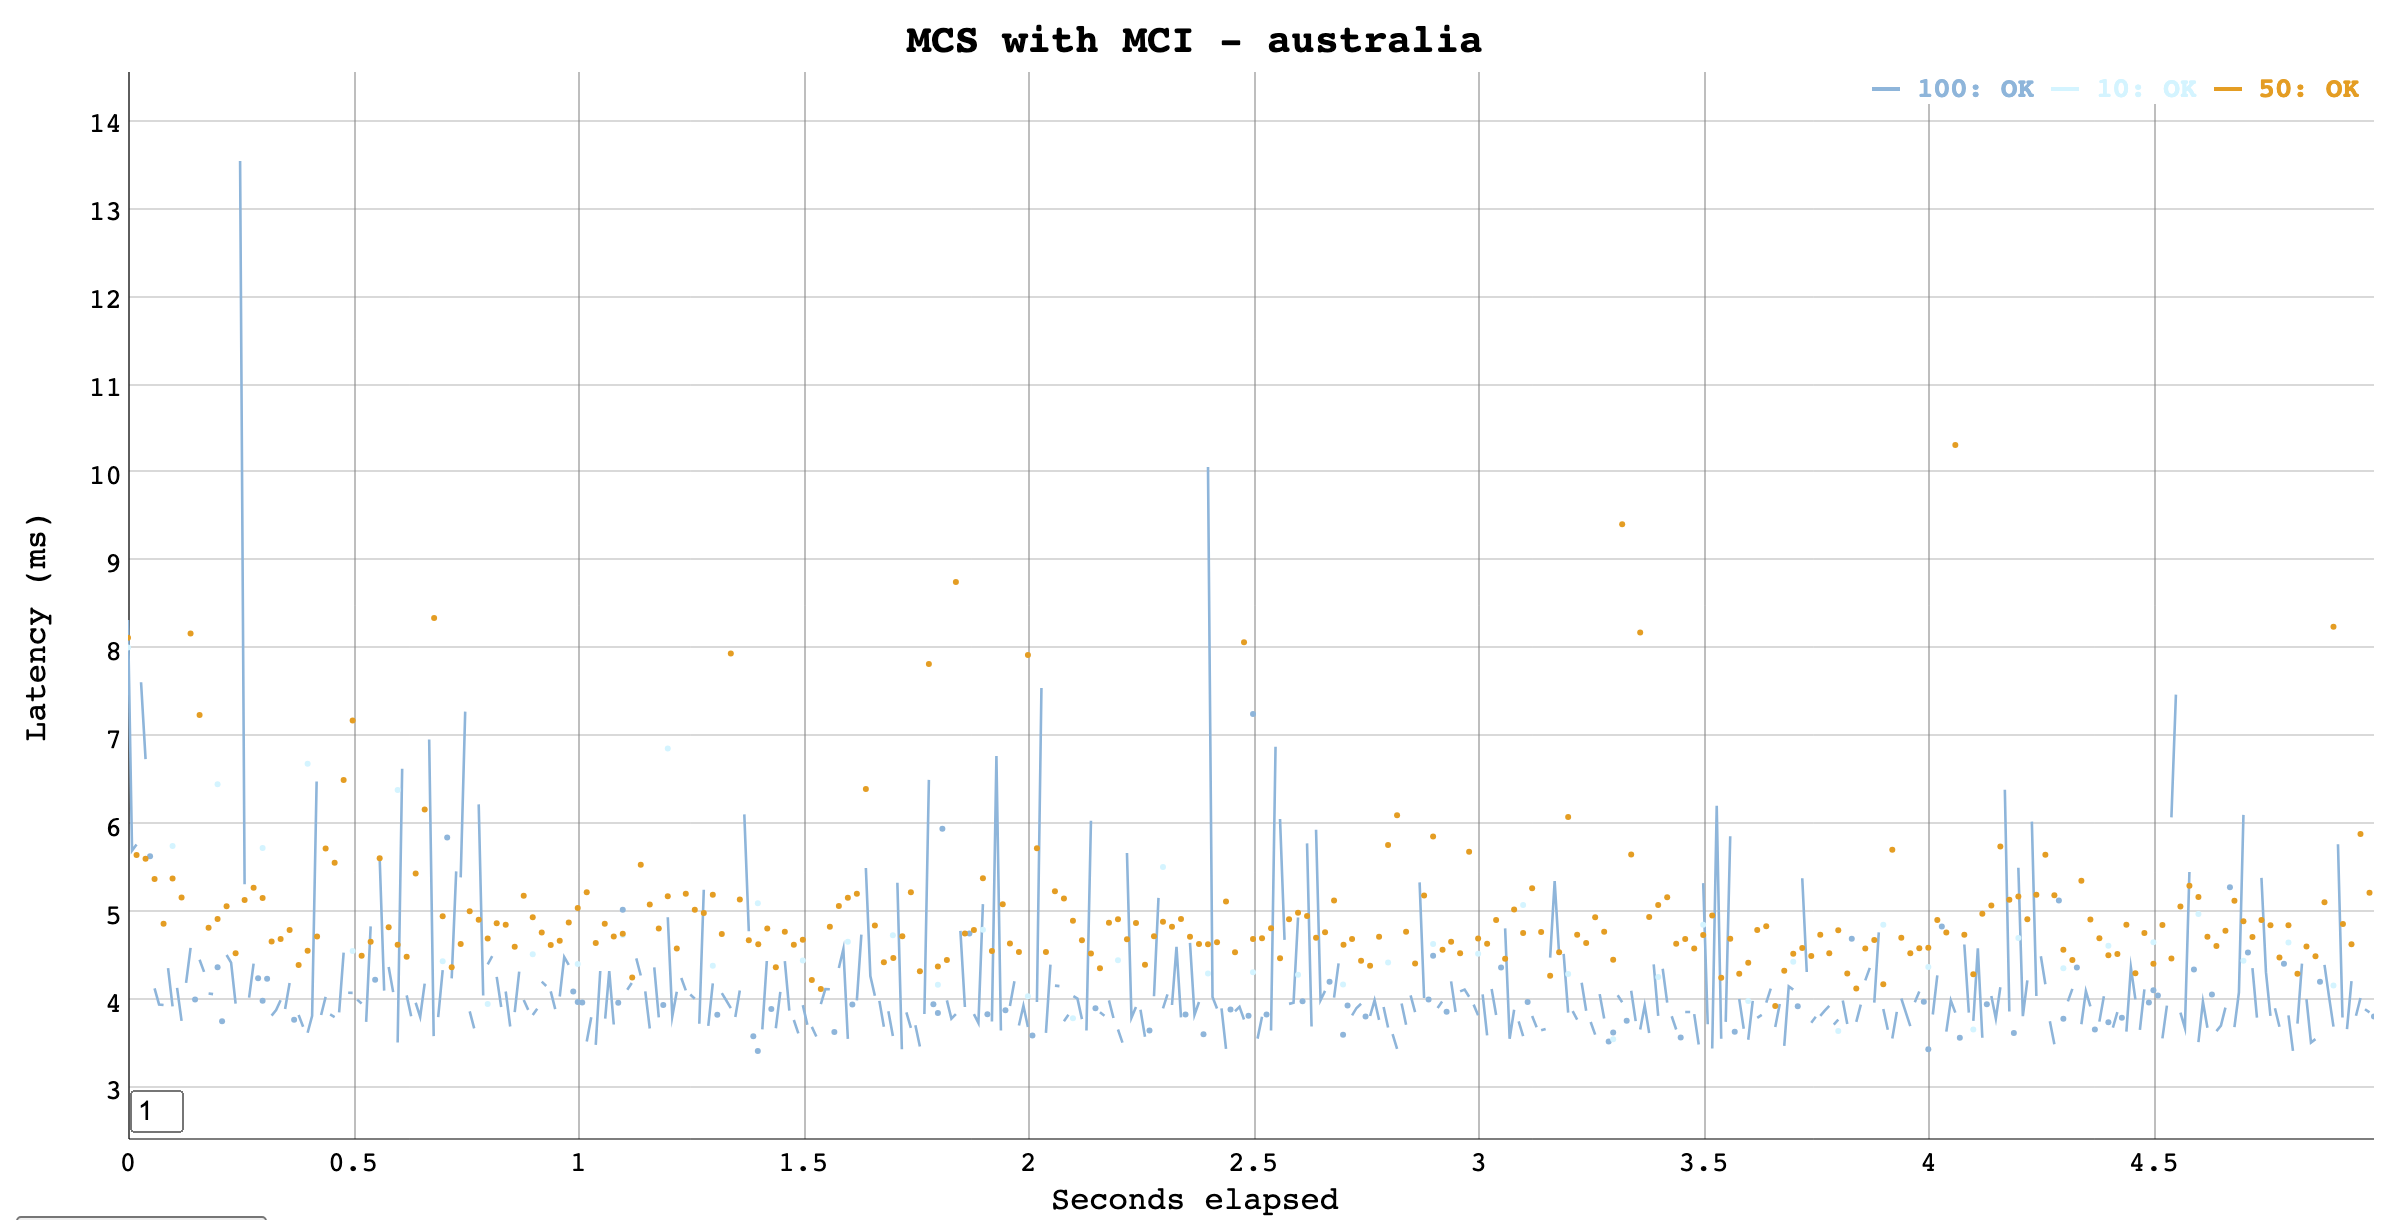
\includegraphics[width=1\textwidth]{assets/plots/mc-aus-1.png}
    \caption{Latency over time of MCS with MCI australia 1.}
	\label{fig:latency-plot-mc-aus-1}
\end{figure}

\begin{figure}
	\centering
	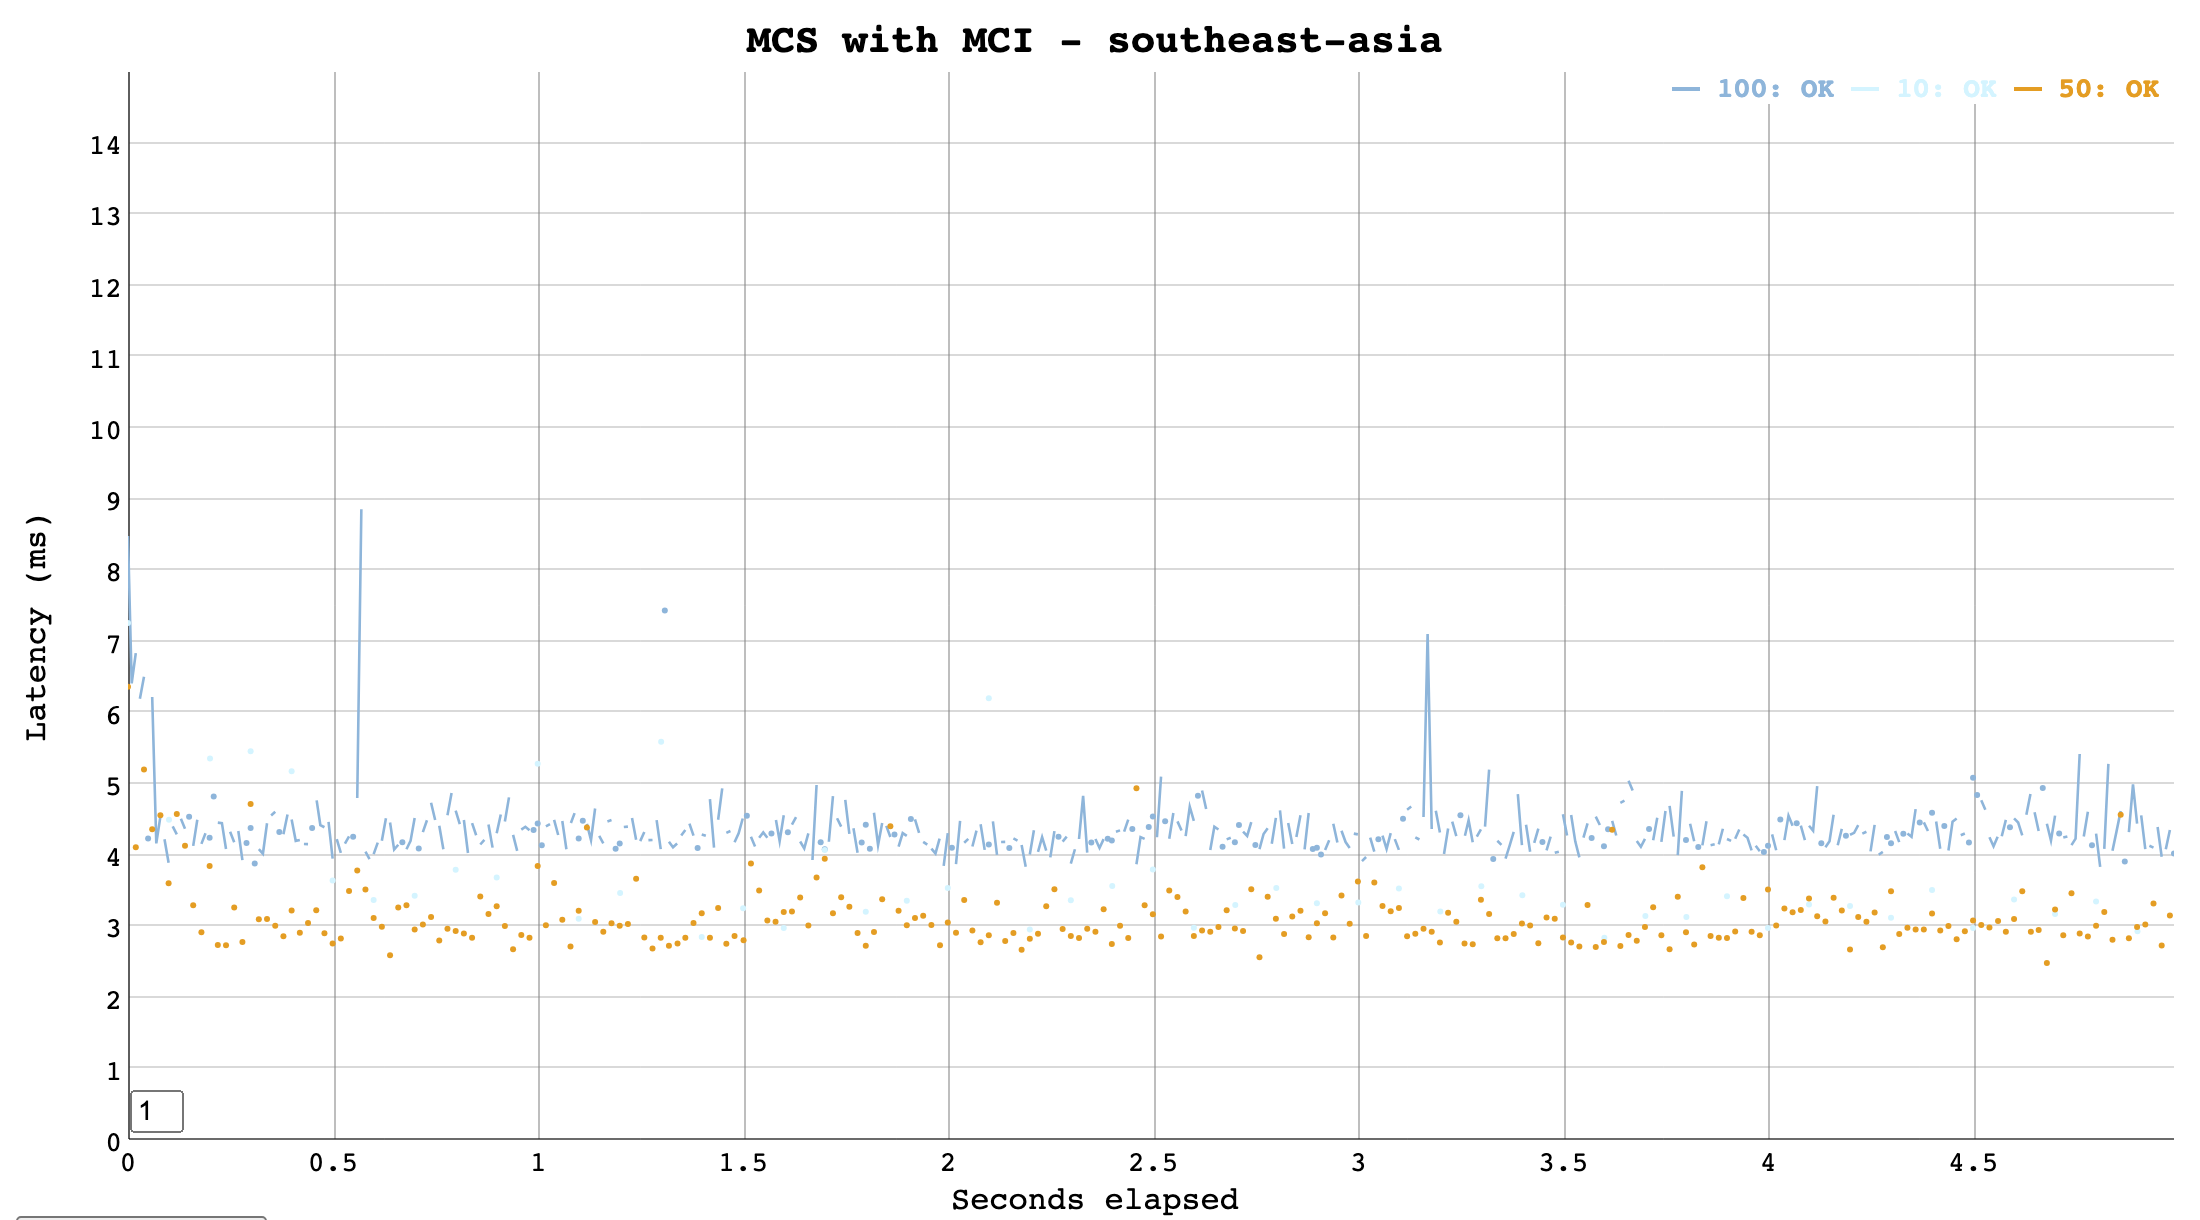
\includegraphics[width=1\textwidth]{assets/plots/mc-sea-1.png}
	\caption{Latency over time of MCS with MCI southeast-asia 1.}
	\label{fig:latency-plot-mc-sea-1}
\end{figure}


To further compare these two approaches, we can compare their latency percentile distribution in order to draw a conclusion. From \autoref{fig:percentile-asm-aus-1-mc-aus-1} and \autoref{fig:percentile-asm-aus-2-mc-aus-2}, it can be seen that Istio / ASM has a lower latency when comparing their 50th and 95th percentile.

\begin{figure}
	\centering
	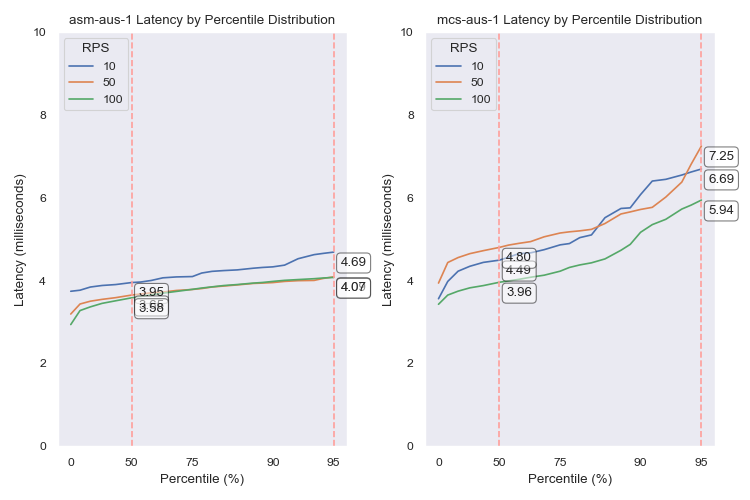
\includegraphics[width=1\textwidth]{assets/plots/percentile-asm-aus-1-mc-aus-1.png}
    \caption{Latency percentile distribution of Istio / ASM and MCS with MCI australia 1.}
	\label{fig:percentile-asm-aus-1-mc-aus-1}
\end{figure}

% \begin{figure}
% 	\centering
% 	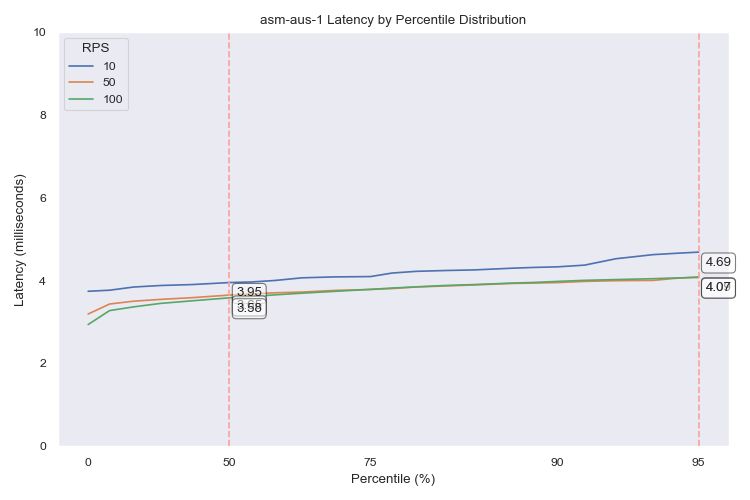
\includegraphics[width=1\textwidth]{assets/plots/percentile-asm-aus-1.png}
%     \caption{Latency percentile distribution of Istio / ASM australia 1.}
% 	\label{fig:percentile-asm-aus-1}
% \end{figure}

% \begin{figure}
% 	\centering
% 	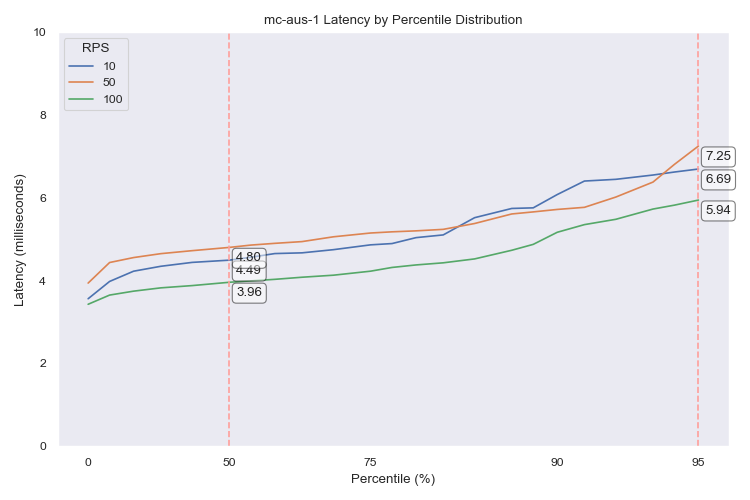
\includegraphics[width=1\textwidth]{assets/plots/percentile-mc-aus-1.png}
% 	\caption{Latency percentile distribution of MCS with MCI australia 1.}
% 	\label{fig:percentile-mc-aus-1}
% \end{figure}

\begin{figure}
	\centering
	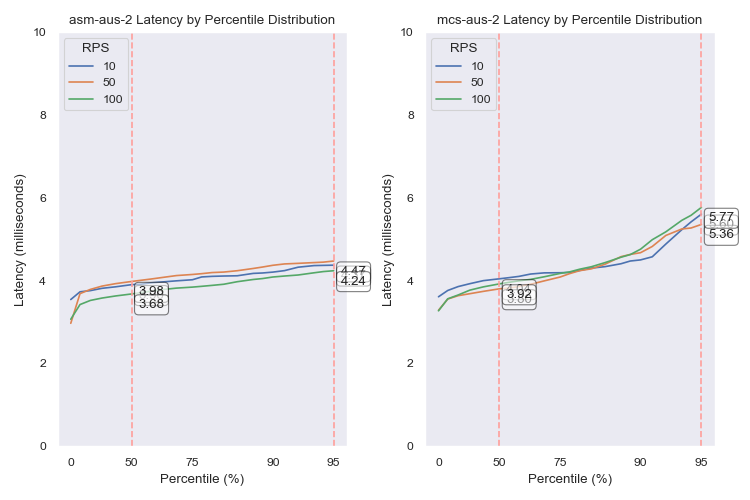
\includegraphics[width=1\textwidth]{assets/plots/percentile-asm-aus-2-mc-aus-2.png}
    \caption{Latency percentile distribution of Istio / ASM and MCS with MCI australia 2.}
	\label{fig:percentile-asm-aus-2-mc-aus-2}
\end{figure}

% \begin{figure}
% 	\centering
% 	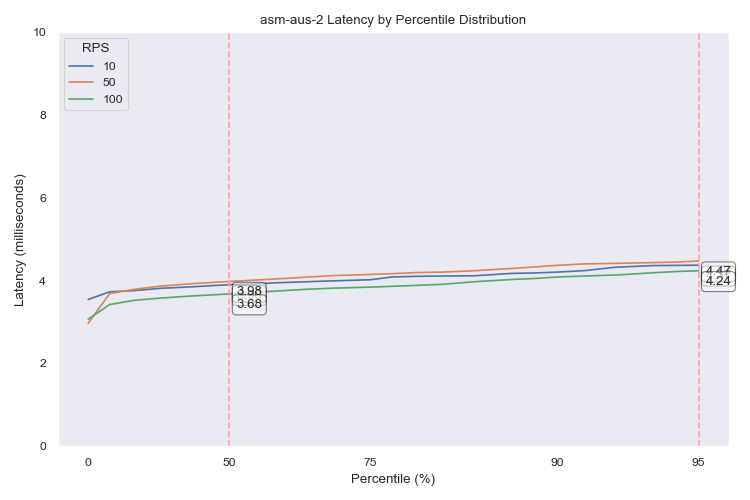
\includegraphics[width=1\textwidth]{assets/plots/percentile-asm-aus-2.png}
%     \caption{Latency percentile distribution of Istio / ASM australia 2.}
% 	\label{fig:percentile-asm-aus-2}
% \end{figure}

% \begin{figure}
% 	\centering
% 	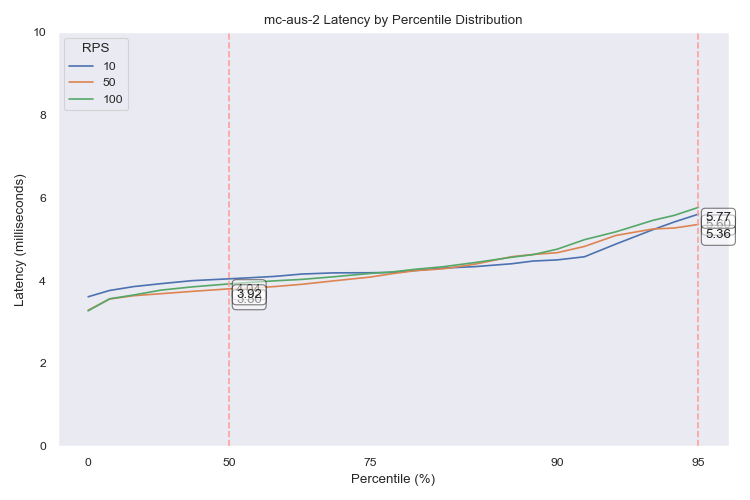
\includegraphics[width=1\textwidth]{assets/plots/percentile-mc-aus-2.png}
% 	\caption{Latency percentile distribution of MCS with MCI australia 2.}
% 	\label{fig:percentile-mc-aus-2}
% \end{figure}

The same result can be seen in the southeast region, where comparing \autoref{fig:percentile-asm-sea-3-mc-sea-3} shows that Istio / ASM has a lower overall latency. We compare the 50th percentile (median) as it is useful to represent what the majority of the response latency looks like. On the other hand, the lower 95th latency percentile and an overall more stable increase compared to the 50th percentile in Istio / ASM tell us that even the small extreme-end of responses that performed worse than normal is still within an acceptable latency.

\begin{figure}
	\centering
	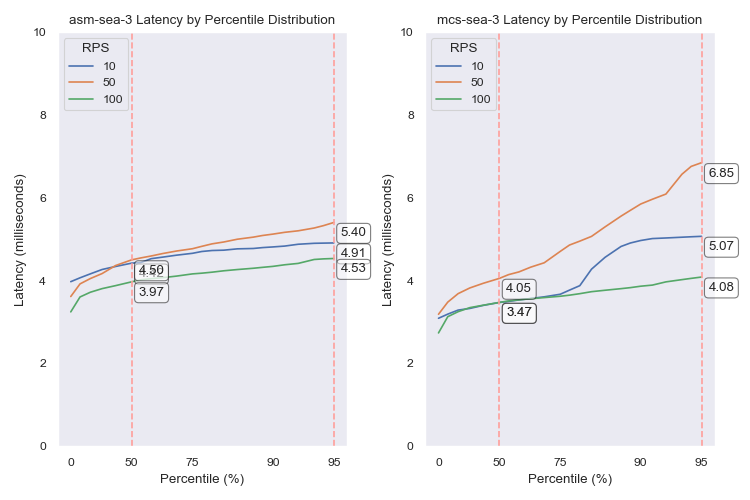
\includegraphics[width=1\textwidth]{assets/plots/percentile-asm-sea-3-mc-sea-3.png}
    \caption{Latency percentile distribution of Istio / ASM and MCS with MCI southeast-asia 3.}
	\label{fig:percentile-asm-sea-3-mc-sea-3}
\end{figure}

% \begin{figure}
% 	\centering
% 	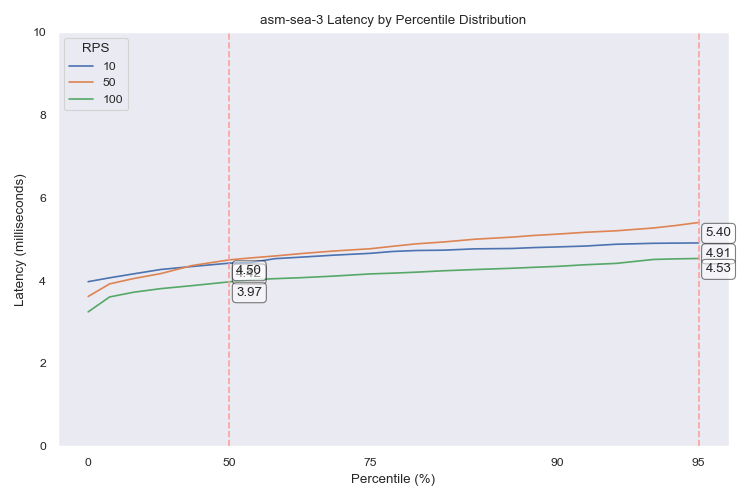
\includegraphics[width=1\textwidth]{assets/plots/percentile-asm-sea-3.png}
%     \caption{Latency percentile distribution of Istio / ASM southeast-asia 3.}
% 	\label{fig:percentile-asm-sea-3}
% \end{figure}

% \begin{figure}
% 	\centering
% 	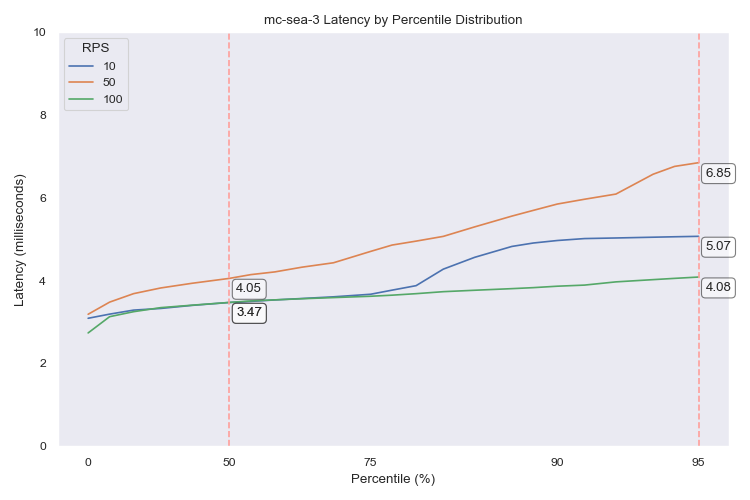
\includegraphics[width=1\textwidth]{assets/plots/percentile-mc-sea-3.png}
% 	\caption{Latency percentile distribution of MCS with MCI southeast-asia 3.}
% 	\label{fig:percentile-mc-sea-3}
% \end{figure}

However, it can't be denied that Istio / ASM suffers from its occasional under-performance, as seen in \autoref{fig:percentile-asm-sea-1-asm-aus-3}, where the jump from the 50th percentile latency to the 95th percentile latency is enormous. This appears to be caused by a combination of  Istio / ASM's slow recovery time and slow failover mechanism, which is not a problem inside an MCS with MCI method.

\begin{figure}
	\centering
	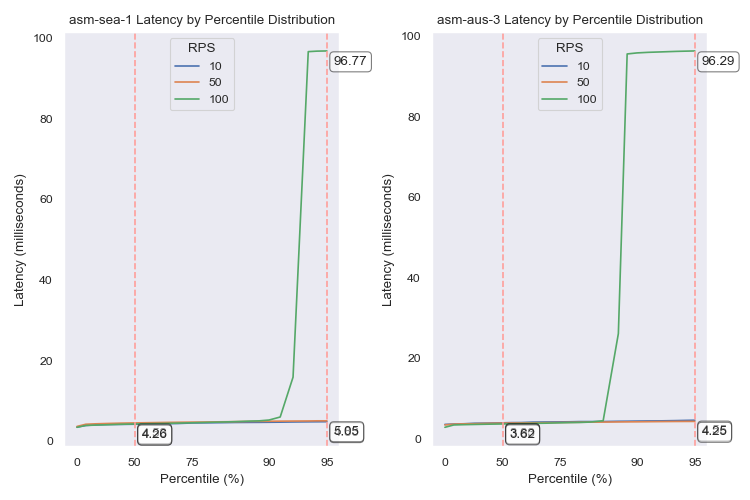
\includegraphics[width=1\textwidth]{assets/plots/percentile-asm-sea-1-asm-aus-3.png}
    \caption{Latency percentile distribution of Istio / ASM southeast-asia 1 and Istio / ASM australia 3.}
	\label{fig:percentile-asm-sea-1-asm-aus-3}
\end{figure}

% \begin{figure}
% 	\centering
% 	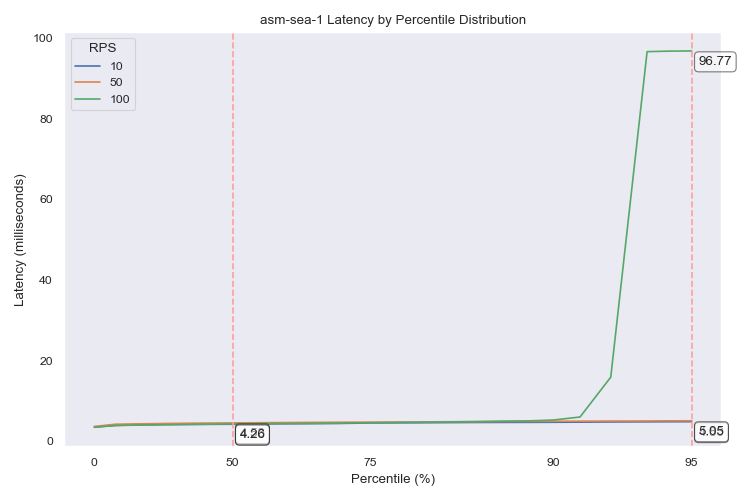
\includegraphics[width=1\textwidth]{assets/plots/percentile-asm-sea-1.png}
%     \caption{Latency percentile distribution of Istio / ASM southeast-asia 1.}
% 	\label{fig:percentile-asm-aus-3}
% \end{figure}

% \begin{figure}
% 	\centering
% 	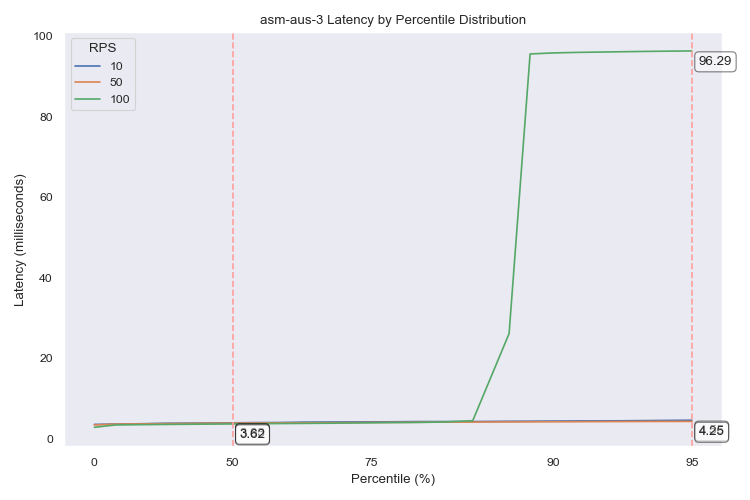
\includegraphics[width=1\textwidth]{assets/plots/percentile-asm-aus-3.png}
% 	\caption{Latency percentile distribution of Istio / ASM australia 3.}
% 	\label{fig:percentile-mc-aus-3}
% \end{figure}

Moreover, comparing the latency's 50th and 90th percentile, as seen in \autoref{tab:multi-cluster-performance-results}, shows that Istio / ASM has the better overall latency, as it has a lower 95th percentile latency in 12 out of 18 experiments with a 1.4-millisecond difference on average compared to the MCS with MCI approach. The MCS with MCI approach has the advantage in 50th percentile performance, however, as it outperforms Istio / ASM 10 out of 18 times with a 10-millisecond difference on average.
% As a result of having a lower 95th percentile latency, Istio / ASM has the better performance. his means that the Istio / ASM approach has a better performance, it is not a significant improvement.


% \clearpage

% Overall, it is true that MCS with MCI has better performance and is a more suitable method for high-traffic scenarios as it consistently handles requests with low-latency responses. This is not to say that Istio / ASM is an objectively worse approach, as it has a diverse amount of features that MCS with MCI doesn't have, such as canary release and rate limiting.

In conclusion, Istio / ASM performs better than MCS with MCI as it is able to handle a wider number of requests with slightly lower latency, despite its outliers. It is advisable to have multiple replicas of each server to avoid long recovery times. Despite this, the difference in median latency is negligible, making MCS with MCI a viable alternative. In addition, an improvement to the failure mechanism can be done by having more clusters to reduce the physical distance between a cluster and its failover destination.

Additionally, it can be seen from \autoref{tab:multi-cluster-performance-results} that Istio / ASM has a lower latency in the australia region while the same can be said with the MCS with MCI method on the southeast-asia region. This is possibly the effect of timezone differences, as the tests were done one after another, which results in different actual local time for each of the region.